% !TeX spellcheck = en_US

%------------------------------%
%&			To Do
%------------------------------%


%------------------------------%
%&			Preambel
%------------------------------%


\documentclass[a4paper,12pt]{article}

\usepackage[a4paper, left = 2.5cm, right = 2cm, top = 2.5cm, bottom = 2.5cm]{geometry} %%% Seitenlayout
\usepackage{amsmath}
%\usepackage{blindtext}  % für grauen Texthintergrund
%\usepackage{bm}
\usepackage{booktabs}
\usepackage{caption} % For table caption
\usepackage[colorlinks=false, pdfborder={0 0 0}]{hyperref}  % Immer vor cleverref
\usepackage{color} % colors for code chunks
\usepackage{float}
%\usepackage{framed} 
\usepackage{graphicx}  % Required for including pictures

\usepackage{listings} %for code chunks 
\usepackage{mathptmx} %% Times new Roman 
\usepackage{microtype}
\usepackage{multicol}
\usepackage[l2tabu, orthodox]{nag}
\usepackage[round]{natbib} % für Zitate 
\usepackage{siunitx}
\usepackage{subcaption} % für subfigure environment
\usepackage{tabularx}
\usepackage{textcomp} 
\usepackage[table]{xcolor}
\usepackage{cleveref} %for clever references which recognize the type of object referenced. See https://en.wikibooks.org/wiki/LaTeX/Labels_and_Cross-referencing

\linespread{1.25} % 1.5 facher Zeilenabstand 
\colorlet{shadecolor}{gray!25} 
\definecolor{dkgreen}{rgb}{0,0.6,0}
\definecolor{gray}{rgb}{0.5,0.5,0.5}
\definecolor{mauve}{rgb}{0.58,0,0.82}
\definecolor{lightgray}{gray}{0.9}
\RequirePackage[l2tabu, orthodox]{nag}



%%%%%%%%%%% Neu in Master 
\usepackage{lscape}  % Die Landscape Umwelt dreht Seiten in die Horizontale
% set indentation length to zero 
\setlength\parindent{0pt} 
% Das caption packet erlaub es global die Einstellungen für Captions (Bild und Tabellen Unter-/Überschriften) zu verändern 
% e.g. Labels dick gedruckt 
\usepackage[labelfont=bf]{caption}
% this refers to the caption text body 
\usepackage[font=small]{caption}



%------------------------------------

\begin{document}

		\pagenumbering{roman}
		
%------------------------------%
%&			TITLE PAGE
%------------------------------%
		
		\begin{titlepage}
			
			\begin{center}
				
				\vspace*{3cm}
							
				%------------------------------%
				%&			TITLE
				%------------------------------%
				
				\begingroup
					% Topline 
					\rule{\textwidth}{1.6pt}\vspace*{-\baselineskip}\vspace*{2pt} 							
					\rule{\textwidth}{0.4pt} 	
					%whitespace above title															
					\vspace{.1em} \\	
					%Title														
					\textbf{\LARGE Model-based multivariate approaches in community ecology}\\	
					% Whitespace below the title
					\vspace{0.25\baselineskip} 
					%Bottomline
					\rule{\textwidth}{0.4pt}\vspace*{-\baselineskip}\vspace{3.2pt} 
					\rule{\textwidth}{1.6pt} 
				\endgroup
				
				%------------------------------%
				%&			AUTHOR
				%------------------------------%
				
				% Distance to Title 
				\vspace{2.5em}
				
				\begingroup
					by\\
					\Large
					 Jonathan Frederik Jupke \\[.5em]
					\normalsize
					Martin-Luther-Stra{\ss}e 41\\
					76829 Landau \\
					 Student ID: 212202111 \\
					jupk7193@uni-landau.de \\
				\endgroup
				
				%------------------------------%
				%&		Supervisors
				%------------------------------%
				
				% Distance to Authors 
				\vspace{2.5em}
				
				\begingroup
					SUPERVISION\\
					\Large
					 Prof. Dr. Ralf Sch{\"a}fer\\
					 Dr. Mira Kattwinkel\\
				\endgroup
				
				\vfill

				%------------------------------%
				%&		Institut
				%------------------------------%
			
				\begingroup
					\small
					Master Thesis for the study program MSc. Environmental Sciences\\
					Fachbereich 7: Natur- und Umweltwissenschaften \\
					Universit{\"a}t Koblenz-Landau
				\endgroup
				
				\vfill
				
				7\textsuperscript{th} September 2018
				
				
			\end{center}     	
		\end{titlepage}
		
		\newpage
%-------------------------------
			
%------------------------------%
%&	DECLARATION OF AUTHORSHIP
%------------------------------%
		
		%Header
		\huge
		\textbf{Declaration of Authorship}\bigskip\\
		
		%Text
		\normalsize
		\noindent „Hiermit best{\"a}tige ich, dass die vorliegende Arbeit von mir selbst{\"a}ndig verfasst wurde und ich keine 
		anderen als die angegebenen Hilfsmittel -- insbesondere keine im Quellenverzeichnis nicht benannten Internet - Quellen --
		benutzt habe und die Arbeit von mir vorher nicht in einem anderen Pr{\"u}fungsverfahren eingereicht wurde.“\bigskip\bigskip\\
		
		%Subscriptionline
		\noindent\begin{tabular}{ll}
			\makebox[2.5in]{\hrulefill} & \makebox[2.5in]{\hrulefill}\\
			Jonathan F. Jupke & Date, Location\\[8ex]% adds space between the two sets of signatures
			
		\end{tabular}	

		\newpage	
%-------------------------------
		
%------------------------------%
%&		Acknowledgements
%------------------------------%
	
		% Header
		\huge
		\textbf{Acknowledgements}\bigskip\\
		
		% Text
		\normalsize
		I would like to thank Prof. Sch{\"a}fer for proposing this thesis topic, helping me through the inevitable road bumps and pushing the simulation process into a productive direction. 
		%
		Further, I owe many thanks to Isabel M{\"u}ller, Sebastian Scheu, Artem Fischbein and Alisa Bamberg for proofreading the thesis.
		%
		Their suggestions have provided valuable input. 
		%
		Lastly, I would like to thank Guillaume Blanchet and Matri Anderson, who even though not directly involved in this work, patiently answered my emails. 
		
		
		\newpage	
%%-------------------------------

		\tableofcontents
		\thispagestyle{empty}

		\newpage
%%%%%%%%%%%%%%%%%%%%%%%%%%%%%%%%%%%%%%%%%%%%%%%%%%%%%%%%%%%%%%%%%%%%%%%%%%%%%%%%%%%%%%%%%%%%%%%%%%%%%%%%%%%%
	\pagenumbering{arabic}
	% !TeX spellcheck = en_US

%------------------------------%
%&			To Do
%------------------------------%


\section{Introduction}

	%------------------------------%
	%&			Erste Absatz:
	%&	Eternal Question + Statisticians point of view 
	%------------------------------%

	Which environmental gradients drive the changes in species abundances and community composition?
	%
	This is one of the oldest questions in ecology \citep[e.g.][]{Clements1907}  and the prospect of humans altering their surroundings at an unprecedented rate endows it with a new urgency \citep{pacifici2015assessing}.
	%
	To answer 	it, ecologists typically record the abundance or occurrence of different taxa and several environmental variables (e.g. precipitation or exposure to stressors), at different sites.
	%
	This results in a sites-by-species matrix $\mathbf{Y}$ containing multivariate species abundances, which is then statistically related to  a sites-by-predictor matrix $\mathbf{X}$, containing the environmental variables.
	%
	From a statisticians point of view, $\mathbf{Y}$ has many undesirable properties: 
	correlation within and between variables, 
	e.g. through biotic interactions \citep{morales2015inferring},
	probability distributions other than the normal, 
	more species than sites \citep[\textit{high dimensionality}, especially in DNA Barcoding studies, ][]{cristescu2014barcoding}  
	and many zeros, since most species are commonly absent from most sites (\textit{sparsity}). \\
	
	%------------------------------%
	%&		Zweite Absatz:
	%&	Distance Based + Whats wrong with it
	%------------------------------%
	
	
	Multivariate species abundances are frequently analyzed by means of their distance or dissimilarity matrix \citep[distance-based analysis \textit{sensu}][]{Warton2012}. 
	%
	This approach is popular among ecologists because it is non-parametric and hence distribution-free \citep[e.g.][]{clarke1993non}.
	% question ist schlecht 
	Whether a distance metric is appropriate depends on the properties of the data and the aim of the study, as each metric extracts different information from the raw data. 
	%
	The choice is complicated by the vast amount of available metrics \citep[see][]{Legendre2012} and contradicting recommendations \citep[][]{faith1987compositional}.
	%
	Deploying a distance metric, one also implicitly assumes a mean-variance relationship in the data. For example, the Minkowski distances (e.g. Manhattan and Euclidean) assume a constant variance across all mean values \citep{TerBraak1988}.  
	%
	However, species abundances often show a quadratic mean-variance relationship \citep{routledge1991taylor, yamamura1999transformation}.
	%
	Miss-specifying the relationship by choosing an improper distance metric can lead to erroneous conclusions about one's data, as was shown by \citet{Warton2012}.
	%
	An alternative to distance-based analysis, that avoids this issue, is the model-based approach.\\ 
 
	%------------------------------%
	%&		Dritte Absatz:
	%&	Model Based Approach
	%------------------------------%


	The model-based approach to multivariate data analysis entails explicitly specifying a statistical model of the process that generated the observed data \citep{Warton2015a}.
	%
	This includes the mean-variance relationship, which can be adjusted to the properties of the data.
	%
	Despite their ubiquity in univariate analyses, model-based approaches have long been uncommon in multivariate ecological analyses.
	%
    However, advances in statistical theory and computation power have led to a surge of models for multivariate abundance data. 
	%
	Recent examples include \textit{Hierarchical Modeling of Species Communities} \citep[HMSC,][]{Ovaskainen2017}, \textit{Generalized Joint 
	%
	Attribute Modelling} \citep[GJAM,][]{Clark2017} and \textit{multivariate Generalized Linear Models} \citep[GLM$_{mv}$,][]{Warton2012}.\\
	
	%------------------------------%
	%&		Vierte Absatz:
	%&			GLMmv
	%------------------------------%
	
	In GLM$_{mv}$, a separate univariate GLM is fit to each taxon, each model using the same predictors. 
	%
	Univariate GLMs are a powerful and flexible method. 
	%
	They are strongly advocated for the analysis of count or occurence data as they can handle different residual distributions and mean-variance relationships \citep{OHara2010, Warton2011, Szocs2015_b}.
	%
	Extending them to multi-species abundance data was thus a natural starting point for multivariate model-based analyses \citep{Warton2012}.
	%
	The univariate models are combined by  summing their test statistics, which enables the researcher to draw conclusions about the whole community.
	%
	GLM$_{mv}$ were one of the earlier multivariate models with an easy-to-use implementation \citep[in the \textit{mvabund} R-package, ][]{Wang2018} and  
	since their introduction they have gained traction within the ecological community (244 citations according to the Web of Science as of 24.04.2018). 
	%
	To my knowledge, the simulations of \citet{Warton2012} remain the only test of GLM$_{mv}$ with simulated data until now.
	%
	\citet{Szocs2015} tested GLM$_{mv}$ with data from ecotoxicological mesocosm studies, and found that they performed better or at least as well as commonly used methods (Principal Response Curves).
	%
	They also emphasized the need for further simulation studies on GLM$_{mv}$.\\

	%------------------------------%
	%&		5. Absatz:
	%&		Aim of the Study
	%------------------------------%
	
	The aim of this study is to test the ability of four statistical methods to determine which environmental gradients drive the changes in sets of simulated multivariate abundance data. 
	%
	The performance of GLM$_{mv}$ will be compared to \textit{Distance Based Redundancy Analysis} (db-RDA), \textit{Canonical Correspondence Analysis} (CCA) as well as \textit{Constrained Additive} and \textit{Quadratic Ordination} (CAO/ CQO).

	%------------------------------%
	%&		6. Absatz:
	%&		Other Methods
	%------------------------------%
	
	% db-RDA
	db-RDA is a distance-based analysis. 
	%
	It calculates an ordination on the distance matrix of the sites-by-species  matrix $\mathbf{Y}$ constrained by the environmental variables $\mathbf{X}$ \citep{Legendre1999, AndersonMati2003}.
	%
	db-RDA was highlighted by \citet{Szocs2015}, because the possibility to use asymmetrical distance metrics and avoid the \textit{double-zero problem } \citep{Legendre2012} makes them attractive for sparse data sets. 
	% CCA
	CCA and CQO are both solutions to Constrained Gaussian Ordination (CGO), in which species are expected to respond unimodally to latent gradients that are linear combinations of environmental variables \citep{gauch1974ordination}. 
	%
	CCA is an algorithmic solution (neither distance- nor model-based), that is based on the findings of \citet{TerBraak1986}. 
	%
	He showed that the maximum likelihood estimation of CGO for Poisson distributed counts can be approximated by correspondence analysis, given that a set of restrictive assumption hold (see section 2.4). 
	%
	CCA is one of the most widely used statistical techniques in ecology, with the essential papers having accumulated over 3000 citations \citep{Braak2014}.
	% CAO/ CQO
	CQO is the maximum likelihood solution to CGO \citep{Yee2004}. 
	%
	It uses an extension to GLM, \textit{Vector Generalized Linear Models} \citep[VGLM,][]{yee1996vector}, to estimate model parameters and is hence model-based. 
	%
	\citet{Yee2006} proposed CAO as a modification to CQO, that uses additive instead of linear models and is thus more flexible and data-driven. \\
	



	\newpage 
%%%%%%%%%%%%%%%%%%%%%%	
	% !TeX spellcheck = en_US


\section{Material and Methods}

	%------------------------------%
	%&		Simulations 			
	%------------------------------%

	\subsection{Simulations}
		Species abundances were simulated as counts, which is the most widely used abundance measure \citep{Warton2008}.
		%
		They responded to an environmental gradient with one of four different response types: unimodal (\textit{uni}), linear (\textit{li}), logistic (\textit{lo}) and bimodal (\textit{bi}).
		%
		Even though all gradients are linear, a gradient to which species respond unimodally will be called unimodal itself, for the sake of readability.\\
	
		%------------------------------%
		%&		Notation 				
		%------------------------------%

		In the remainder, the following notation is used. 
		%
		$\mathbf{Y}$ is a $N \times S$ matrix of responses, in this case, the abundances of $S$ species, $ s= 1\ ...\ S$, at $N$ sites, $ n = 1\ ...\ N$.
		%
		$\mathbf{X}$ is a $N \times M$ matrix of predictors, here, $M$ environmental variables, $m = 1\ ... \ M$. \\
	
		%------------------------------%
		%&		Responses				
		%------------------------------%
		
		Unimodal responses were simulated using the Gaussian Response Model \citep{GauchJr1972} expanded to multiple gradients (Eqn. \ref{eq:GaussianResponseModel}).
		%
			\begin{equation} \label{eq:GaussianResponseModel}
					y_{s,n} = \prod_{m}^{M_{Uni}} c_{s,m} \times exp\bigg(-\frac{(x_{m,n} - u_{s,m})^2}{2t^2_{s,m}}\bigg)		
			\end{equation}
		%	
		In this equation, $u_{s,m}$ is the position of the optimum (i.e. the point with the highest abundance) of species $s$ along the gradient $m$, $t_{s, m}$ is the tolerance of species $s$ toward the gradient $m$ and determines the width of the curve and $c_{s,m}$ is the maximum abundance of species $s$ on gradient $m$. 
		%
		$M_{uni}$ is the number of unimodal gradients. \\
		%
		Linear responses were simulated by multiplying the gradient value with a coefficient $\beta$ (Eqn. 2).
		%
		\begin{equation}
		 				y_{s,n} = \prod_{m}^{M_{lin}} x_{m,n} \times \beta_{s,m}
		\end{equation}
		%
		Logistic responses were simulated using the Verhulst-equation \citep[][Eqn. \ref{eq:Verhulst}]{verhulst1838notice}.
		\begin{equation} \label{eq:Verhulst}
						y_{s,n} = \prod_{m}^{M_{log}}  \frac{c_{s,m}}{1+ exp(-k_{s,m}(x_{0\ s,m}-x_{m,n}))}
		\end{equation}
		%
		Here, $k$ determines the steepness of the curve and $x_0$ is the x-value of the sigmoids midway point.\\ 
		
		%
		Bimodal data were simulated by adding two unimodal models with different optima.
		%
		The total abundance of species $s$ at site $n$ was calculated by multiplying the abundances for individual gradients. \\
		
		%------------------------------%
		%&		The Gradients	
		%------------------------------%
		Species were simulated to respond to two environmental gradients: \textit{env1} and \textit{env2}.
		%
		All species show the same response type towards the same gradient, but response types can differ between gradients. 
		%
		Figure \ref{fig:bivariateExample} shows three example communities.\\
	
		This setup allows for ten distinct combinations of response types, including those where the species' response types are the same for both graidents (e.g. Figure \ref{fig:bivariateExample1}).  
		%
		The combinations are referred to by the concatenations of their abbreviated response types, e.g. \textit{Lo-Bi} for a community that responds logistically to the first and bimodally to the second gradient, like the one depicted in Figure \ref{fig:bivariateExample3}. 
	
	
		%------------------------------%
		%&		Figure: 3d Response shapes	
		%------------------------------%
		\begin{figure}[h!]
			
			\begin{subfigure}{0.3\textwidth}
				\centering
				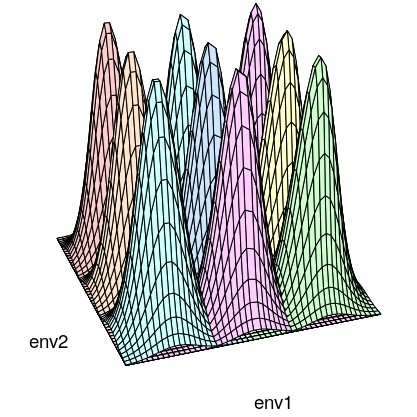
\includegraphics[width=1\linewidth]{../02_Figures/Uni-Uni_Model}
				\caption{\textit{Uni-Uni}}
				\label{fig:bivariateExample1}
			\end{subfigure}
			\begin{subfigure}{0.3\textwidth}
				\centering
				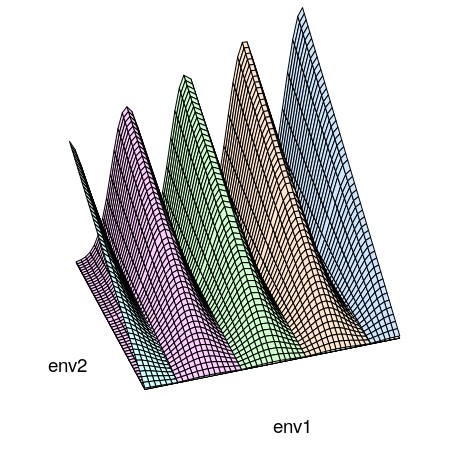
\includegraphics[width=1\linewidth]{../02_Figures/Uni-Li_Model}
				\caption{\textit{Uni-Li}}
			\end{subfigure}
			\begin{subfigure}{0.3\textwidth}
				\centering
				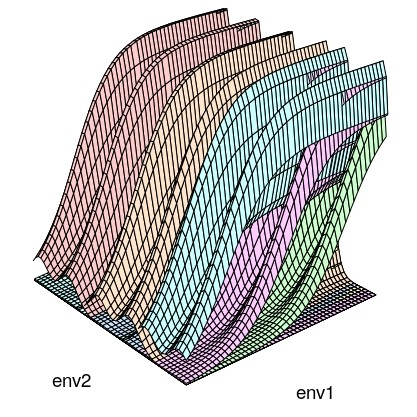
\includegraphics[width=1\linewidth]{../02_Figures/Lo-Bi_Model}
				\caption{\textit{Lo-Bi}}
				\label{fig:bivariateExample3}
			\end{subfigure}
			\caption{Simulated abundance responses along two environmental gradients. Model names are concatenations of abbreviated response types, i.e. (\textbf{a}) unimodal-unimodal, (\textbf{b}) unimodal-linear and (\textbf{c}) logistic-bimodal. The vertical axis indicates abundance as counts.
				Each example consists of 2500 samples.}
			\label{fig:bivariateExample}
		\end{figure}
	
		%------------------------------%
		%&		Model MISC	
		%------------------------------%
		
		The models \textit{Uni-Li}, \textit{Li-Lo} and \textit{Li-Bi} include five species.
		%
		All other models consist of nine species.
		%
		They are numbered as follows: for models with nine species, they are numbered first on \textit{env1} from low to high and then on \textit{env2}, i.e. species one's optimum is at a low value for \textit{env1} and \textit{env2} (blue in Figure \ref{fig:bivariateExample1}) and species nine's optimum has a high value in both \textit{env1} and \textit{env2} (pink in Figure \ref{fig:bivariateExample1}). 
		%
		For models with five species, they are numbered from low optimum values to high ones on \textit{env1}.
		%
		More details on the parameterization of the models are provided in Table \ref{tab:SimDet} in the Supplementary Materials.
		%
		The two gradients span a grid of 100 $\times$ 100 points for which abundances were simulated. 
		%
		This data set was sampled at equally spaced sampling points and with varying sample sizes (see Table \ref{table:classes}). 
		%
		Noise variables were simulated from a standard normal distribution, scaled to the same magnitude as the environmental gradients and restricted to be orthogonal to them and to each other.  
		%
		For each of the ten combinations of response types, four different classes of models were simulated differing in the sample size and number of noise variables. 
		%
		The four classes are shown in Table \ref{table:classes}. \\
	
		%------------------------------%
		%&	Table: Model classes
		%------------------------------%
		\begin{table*}[h!]
			\begin{center}
			
				\caption{The four model classes. Classes differ in number of samples taken and on the number of noise variables.}
				\begin{tabular}{@{}lll@{}}
					
					\toprule
					 Class & Sample size & Noise variables  \\
					\hline
					1 & 100 & 1 \\
					2 & 100 & 5 \\
					3 & 225 & 5 \\
					4 & 25  & 5 \\	
					\bottomrule
				\end{tabular}
				
				\label{table:classes}
			\end{center}
		\end{table*}
	
	
		Finally, each model was run using three different seeds for random number generation. 
		%
		In total, this gives 120 simulated communities. 
		%
		For a flow chart that visualizes the simulation process see Figure \ref{fig:flowchart_simulation}.\\
		
		%------------------------------%
		%&		Figure: Flowchart 	
		%------------------------------%
		\begin{figure}[h!]
			\centering
			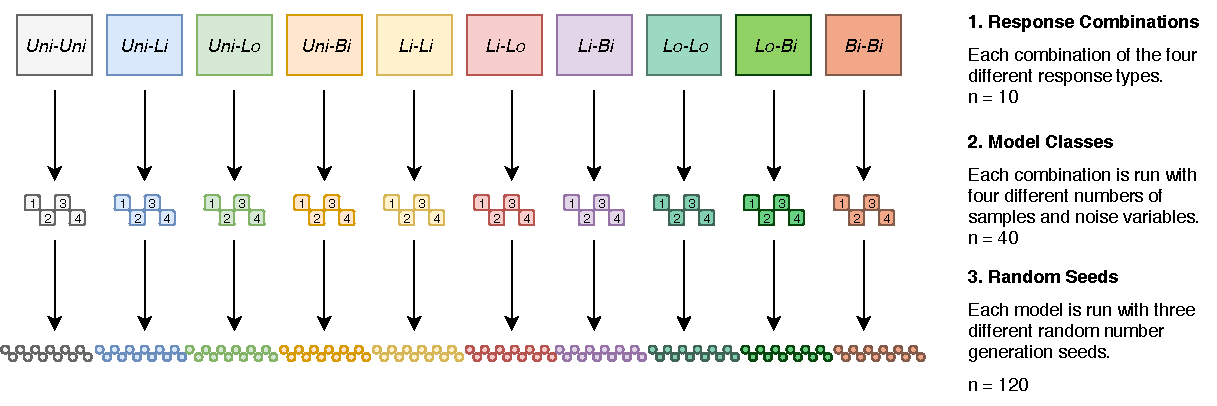
\includegraphics[width=1\linewidth]{../02_Figures/Flowchart}
			\caption{Flowchart of the simulation process. All possible combinations of the four response types unimodal (uni), linear (li), logistic (log) and bimodal (bi) were run in four different classes. The classes differed in how many samples are taken from the simulated community and in how many noise variables are included (see Table \ref{table:classes}).}
			\label{fig:flowchart_simulation}
		\end{figure}
	

		%------------------------------%
		%&	p-Werte 	
		%------------------------------%
		I used \textit{p}-values to compare the method's performances. While their use has been repeatedly criticized for over 50 years \citep[e.g.][]{rozeboom1960fallacy}, they provide a valuable means to compare methods as disparate as those tested herein. 
		%
		Three of the four methods (\textit{viz.} GLM$_{mv}$, db-RDA and CCA) provide \textit{p}-values for the influence of environmental variables on species abundances. Further, the use of \textit{p}-values in ecology and related fields is still wide spread \citep{FIDLER2006} and their performance is thus of practical importance. \\


	%------------------------------%
	%& GLM-MV
	%------------------------------%
	\subsection{Multivariate Generalized Linear Models}

		GLM$_{mv}$s are collections of $S$ separately fitted GLMs. 
		%
		Their likelihood ratios for each environmental variable are summed up to obtain the sum-of-Likelihood-Ratios statistic. 
		%
		This test statistic can provide a multivariate \textit{p}-value, showing whether an environmental variable has a statistically significant effect on the mean community abundance. 
		%
		By summing the likelihood ratios one assumes that species responses are independent of each other. 
		%
		This assumption is relaxed in the hypothesis tests because significance is assessed via row resampling, which preserves the correlation structure. 
		%
		Two alternative, computationally more demanding, test statistics are available: the Wald and the score test statistic. 
		%
		Both explicitly account for correlation between variables, by using Generalized Estimation Equations as proposed by \citet{Warton2011a}.\\ 
		%   
		The effect of each individual species can be assessed by the deviations of the univariate GLMs. 
		%
		Their \textit{p}-values are adjusted to multiple testing by controlling the family-wise type I error rate using a resampling-based version of the \textit{Holm's step-down multiple testing procedure} \citep{Westfall1993}. 
		%
		These adjusted \textit{p}-values tend to be very conservative \citep{Warton2018}. \\
		
		Each model was fit with negative binomial, Poisson, and normal residual distribution and their respective canonical links.
		%
		The fit of the three different models was checked with Dunn-Smith residual-plots and Akaike's Information Criterion \citep[AIC, ][]{akaike1974new}.
		%
		Hypothesis tests for the best fitting model were conducted using the likelihood ratio statistic, each model was resampled 500 times using the PIT-trap bootstrap procedure \citep{Warton2017}.
		%
		Besides resampling, no adjustment for inter-species correlations was used.\\

	%------------------------------%
	%& db-RDA
	%------------------------------%
	\subsection{Distance Based Redundancy Analysis}

		db-RDA  is the constrained form of Principal Coordinates Analysis (PCoA), an eigenvalue-based ordination conducted on distance matrices.
		%
		In a PCoA, $\mathbf{Y}$ is transformed into a centered distance matrix $\mathbf{D}$.
		% 
		Eigenvectors of $\mathbf{D}$, are scaled to the length of $\sqrt{\lambda_k}$, with $\lambda_k$ being the eigenvalue of the $k^{th}$ eigenvector $u_k$. 
		%
		The scaled eigenvectors are the columns of the principal coordinates matrix $\mathbf{PC}$ \citep{gower1966some}.
		% 
		The $\mathbf{PC}$ matrix is then used as a response matrix in an RDA. 
		%
		The db-RDA preserves the distance metric which was used to calculate $\mathbf{D}$, which can be metric, semi- or non-metric, setting	 the method apart from MANOVA \citep{anderson2001new} and transformation-based RDA \citep{Legendre2001}. 
		%
		However, semi- and non-metric distances can produce negative eigenvalues which entail complex ordination axes. 
		%
		These are problematic as they can not be interpreted in a meaningful way. 
		%
		Adding a constant to the squared dissimilarities can correct this \citep[\textit{Lingoes correction}, ][]{gower1986metric}.
		%
		Hypothesis tests on the significance of individual constrained axes and environmental variables can be conducted using a pseudo-F-Statistic with permuted residuals  \citep{Legendre2011}.
		  	
		The semi-metric percentage difference distance metric was used. 
		%
		It was introduced by \citet{odum1950bird} and is commonly referred to as Bray-Curtis Distance \citep{Legendre2012}.
		%
		It is asymmetric and thus avoids the double zero problem  \citep{Legendre2012} and is generally acknowledged to have desirable properties for species abundance data \citep{bloom1981similarity,faith1987compositional}.
		%
		Hypothesis tests on axes and covariables were conducted with 999 permutations. 

	
	%------------------------------%
	%&  CCA
	%------------------------------%
	\subsection{Canonical Correspondence Analysis} \label{subsec:CCA}
	
		CCA has long been the most common way to estimate the parameters of a CGO, even though it is only an approximation of the maximum likelihood solution. 
		%
		It assumes equal tolerances, equal maximal abundances, uniform distribution of species optima and site scores over the latent variable space and bell-shaped responses \citep{TerBraak1986}. 
		%
		The assumptions are collectively known as the \textit{species packing model}. 
		%
		\citet{Palmer1993}, \citet{Johnson1999} and \citet{Zuur1999} confirmed the validity of the approximation and its robustness towards violations against assumptions of the species packing model in simulation studies.
		%
		Nonetheless, the restrictive assumptions were widely criticized \citep[e.g.][]{Austin1994}. \\
		%
		An iterative algorithm is used to obtain estimates. First, arbitrary values are assigned to the site scores (positions of sites in latent variable space, $\mathbf{Z}$). 
		%
		These are used to calculate the species optima  $u$ (henceforth species scores) as in Eqn. \ref{eq:CCA_species_scores}.
		%
		\begin{equation}\label{eq:CCA_species_scores}
		\mathbf{u} = \mathbf{D}_c \mathbf{Y}^t \mathbf {Z}
		\end{equation}
		%
		Where $\mathbf{u} = (u_1\ ...\ u_S)^t$, $\mathbf{D}_c$ is a diagonal matrix with the abundance of species $s$ across all sites as its $s,s^{th}$ element and $\mathbf{Y}^t$ denotes the transpose of $\mathbf{Y}$.\\
		%
		The species scores are in turn used to calculate the site scores as their weighted average $\mathbf{Z}_{wa}$ (Eqn. \ref{eq:CCA_site_scores}) 
		%
		\begin{equation} \label{eq:CCA_site_scores}
			\mathbf{Z}_{wa} = \mathbf{D}_r^{-1} \mathbf{Y} \mathbf {u}
		\end{equation}
		%
		where $\mathbf{D}_r$ is a diagonal matrix with the abundance of all species at site $n$ as its $n,n^{th}$ element and $\mathbf{D}_r^{-1}$ denotes the inverse of $\mathbf{D}_r$. 
		%
		$\mathbf{Z}_{wa}$ is regressed against $\mathbf{X}$ to obtain the weighted regression coefficient $\alpha$. 
		%
		\begin{equation}\label{CCA_canocical_weights}
		\alpha = (\mathbf{X}^t \mathbf{D}_r \mathbf{X})^{-1} \mathbf{X}^t \mathbf{D}_r \mathbf{Z}_{wa}
		\end{equation}
		%
		Lastly, $\mathbf{Z}$ is calculated as the product of $\mathbf{X}$ and $\mathbf{\alpha}$. 
		%
		This procedure is repeated until convergence. \\
	    
		The distance between sites (scaling 1) or species (scaling 2) in CCA approximates their two dimensional $\chi^2$-distance, i.e. the Euclidean distance between the expected abundances under the null hypothesis, that abundances do not change along environmental gradients, and the actual data.
		%
		The absolute difference between expectation and measurement is known as \textit{total inertia}. 
		%
		The ratio of constrained inertia, i.e. variation that can be explained by constrained axes, and total inertia is a general measure of fit for a CCA.
		%
		The chi-squared-distance is asymmetrical and therefore is unaffected by the double zero problem, but it has been criticized since the same absolute change in a rare species is weighted much stronger than an equal change in an abundant species \citep{greig1983quantitative}. 
		%
		The relation between ecological and chi-squared distance is weaker than in other metrics \citep{faith1987compositional,Legendre2001}.
		%
		The significance tests for axes or environmental variables are calculated using a pseudo-F-Statistic as in db-RDA.
	
	%------------------------------%
	%&  CAO/CQO
	%------------------------------%
	\subsection{Constrained Additive and Quadratic Ordination}

		CQO and CAO are based on VGLMs and their additive counterpart VGAMs, respectively. 
		%
		VGLMs expand GLMs, in that they can encompass multiple response variables, each with a separate linear predictor. 
		%
		The modeled responses can be other parameters than the mean(e.g. the variance) and
		%
		VGLMs are not restricted to residual distributions from the exponential family. \\
		%CAO and CQO are based on vector generalized models. The basic VGLM is given in Eqn. \ref{eq:VGLMbasic}.
		%\begin{equation}\label{eq:VGLMbasic} \tag{2.2.1}
		%\eta_s(\mathbf{x}) = g_s(\theta_s) = \sum_{k = 1}^M \beta_{(s)k}\ x_k  	
		%\end{equation}
		%Where $\eta_s$ is the linear predictor for the $s^{th}$ response variable, $g_s$ is the parameter link function for the parameter $\theta_s$ and $\beta_{(j)k}$ is the regression coefficient for response variable $s$ and covariable $k$.\\
		
		Both methods employ \textit{Reduced Rank VGLMs/ VGAMs} (RR-VGLM/ VGAM). 
		%
		In RR-VGLMs the $M$ environmental variables are reduced to $R$ latent variables $\nu$. 
		%
		Therefore, the design matrix $\mathbf{X}$ and hat matrix $\mathbf{B}$ are each partitioned into two subsets 
		$\mathbf{X} = (\mathbf{x}_1^T,\mathbf{x}_2^T)^T$; $\mathbf{B} = (\mathbf{B}_1^T,\mathbf{B}_2^T)$. 
		%
		$\mathbf{x}_1$ and $\mathbf{B}_1$ contain covariables and corresponding regression coefficients, which do not contribute to the latent variables. 
		%
		In practice, $\mathbf{x}_1$ often only contains the intercept and $\mathbf{B}_1$ is thus a vector of 1s with length $M$. $\mathbf{B}_2$ is reduced to a rank $R$ matrix (with full column rank). 
		%
		This is done by reduced rank regression \citep{Anderson1951, izenman1975reduced}, which determines a low-rank matrix that is an optimal
		approximation of a full rank matrix. 
		%
		Unlike in db-RDA or CCA, the researcher specifies the number of latent variables, i.e. the rank of $\mathbf{B}_2$, \textit{a priori}.
		%
		It is referred to as the rank of the method. \\
		%
		The low-rank matrix $\mathbf{B}_2$ is decomposed into two thin matrices $\mathbf{A}$ and $\mathbf{C}$ (see Eqn. \ref{eq:ReduceB2}).
		
		\begin{equation}\label{eq:ReduceB2}
		\mathbf{B}_2^T = \mathbf{A}\ \mathbf{C}^T	
		\end{equation}
		
		The matrix $\mathbf{C}^T$ contains the constrained coefficients, which act as constants in the linear combination of $\mathbf{x}_2$ that constitutes the latent variables. (cf. Eqn.\ref{eq:ctx2})
		
		\begin{equation}\label{eq:ctx2}
		\mathbf{\nu} = \mathbf{C}^T \mathbf{x}_2	
		\end{equation}
		
		The linear predictor therefore becomes:
		
		\begin{equation}\label{eq:ctx3}
		\eta = \mathbf{B}_1^T \mathbf{x}_1 + \mathbf{A} \mathbf{\nu}	
		\end{equation}
		
		
		CQO is an adaption of RR-VGLMs to ecological data sets.
		%
		It assumes that the response variables show symmetric and bell-shaped responses to the underlying gradients represented by the latent variables.
		%
		To this end, quadratic RR-VGLM of the kind of Eqn. \ref{eq:CQO1} are used.
		
		\begin{equation}\label{eq:CQO1} 
		\eta_s = \beta_{(s)1} x_{(s)1} + \beta_{(s)2} \nu + \beta_{(s)3} \nu^2	
		\end{equation} 
		
		The response curve is unimodal for all $\beta_3 < 0$.
		%
		CQO does not assume the species packing model of the CCA.
		%
		Three different assumptions can be made concerning the tolerances: (i) equal tolerances, (ii) unequal tolerances and (iii) identity tolerances.
		% 
		The equal tolerance assumption expects tolerance matrices $\mathbf{T}$ to be equal for all species $\mathbf{T}_1 = \mathbf{T}_2 = ... = \mathbf{T}_S$.
		%
		With the unequal tolerances assumption, the tolerance for each species is estimated separately.
		% 
		For one species $T_s \equiv I_R$, as long as any species has a positive-definite tolerance matrix. 
		%
		Lastly, identity tolerance sets $T_s \equiv I_R$ for all species. 
		%
		This implies the equal tolerance assumption.  
		% 
		Equal or identity tolerance models are expected to be faster and easier to interpret but unequal tolerance models should fit the data better \citep{yee2015vector}.\\
		% 
		In a CAO the assumptions of symmetric bell shaped responses is relaxed by using a smooth function for $\nu$. 
		%
		The RR-VGAM can be conceptualized as fitting a generalized additive model for each species against the latent variables.
		%
		As of now, the method is still limited in its capabilities \citep{Yee2006}.
		%
		Only rank-1 models can be fitted and only to Poisson or binary responses.  
		%
		\citet{Yee2006} advocates to use CAO for exploratory data analysis and CQO for inference, akin to using Generalized Additive Models as a diagnostic tool before running GLMs \citep{Hastie2008}.\\
		  
		 
		CAO and CQO were run with Poisson residual distribution and the canonical log-link function.
		%
		The effective nonlinear degrees  of freedom was set to 1.5 as suggested by \citet{yee2015vector}.
		%
		Constrained coefficients on the first axis were restricted to be positive. 
		%
		Each model was run ten times and the solution with the lowest deviance was used to safeguard against local solutions.
		% 
		% General Info - absolute values 
		For the calculation of mean values and standard deviations the constrained coefficients of CAO and CQO were transformed to absolute values. 
		%
		To asses the influence of environmental variables on the latent variable, the algebraic sign is not of interest, since it only shows the directionality of the former on the latter.
		%
		Rank-1 models were run for CAO, rank-1 and rank-2 models with all three tolerance settings for CQO. 
		%
		The optimal number of ranks was found to be two for all models, determined by the AIC as proposed by \citet{yee2003reduced}. \\
		
		
	\subsection{Software}
		All simulations and analyses were done in R 3.4.4 \citep{RCT2018}.
		%
		GLM$_{mv}$s were conducted with mvabund 3.13.1. \citep{Wang2018}, db-RDA and CCA with vegan 2.5-2 \citep{Oksanen2018} and CAO/CQO with VGAM 1.0-5 \citep{Yee2018}. 
		%
		R-scripts for the simulations as well as the analyses are available on \href{https://github.com/JonJup/Master-Thesis.git} {GitHub} (https://github.com/JonJup/Master-Thesis)


	
	
% !TeX spellcheck = en_US
%	TODO	-	Outlier beschreiben 
 
\section{Results}

	%------------------------------%
	%& 			In General 			
	%------------------------------%

		%------------------------------%
		%& 		Konvergenz				
		%------------------------------%
	
		CCA and db-RDA successfully ran for all models, while GLM$_{mv}$s and CAO/CQO had convergence problems. 
		%
		They mostly occurred with class four methods, which have a low sample size to parameter ratio (see Table \ref{table:classes}). 
		%
		For GLM$_{mv}$s non-convergence was determined by run time. 
		%
		Models that ran more than 18 hours were aborted and classified as non-converging.
		% 
		Non-convergence of GLM$_{mv}$s occurred for all class four and one class two (Uni-Uni) model. 
		%
		CAO failed to converge for all level four models of \textit{Uni-Li} and \textit{Uni-Bi}; CQO for  all class four models of \textit{Uni-Bi}, for unequal and identity tolerance models of \textit{Uni-Uni} and for unequal tolerance models of \textit{Uni-Lo, Lo-Bi} and \textit{Bi-Bi}.\\

		%------------------------------%
		%& 		Runtime 				
		%------------------------------% 
	
		$GLM_{mv}$ was the slowest method. 
		%
		For a class three \textit{Uni-Uni} model the GLM$_{mv}$ ANOVA ran 03:13 h;
		db-RDA 1.7 min for axis and 4 s for terms; 
		CCA 2 s for axis and $< 1s $ for terms; 
		CAO 9 min  and in COQ 28 s for equal tolerance, 9 s for unequal tolerance and 6 s for identity tolerance (on an Ubuntu 18.04 machine with 64-bit, 8 GB RAM and 1.6 GHz).

		%------------------------------%
		%& 		Verweise 				
		%------------------------------%  
	
		Means and standard deviations of \textit{p}-values of GLM$_{mv}$, db-RDA and CCA for all covariables are shown in Table \ref{table:results1}.
		
		I refer to the Supplementary Materials for tables of covariable and axes \textit{p}-values at the level of response combinations or classes (Table \ref{tab:SMGLM1} - \ref{tab:ccasm4}), CCA inertias (Table \ref{tab:smcca5} and \ref{tab:smcca6}), Canonical Coefficients of CAO (Table \ref{tab:caosm1} and \ref{tab:caosm2}) and CQO (Table \ref{tab:cqosm1} - \ref{tab:cqosm3}) as well as selected ordination diagramms (Figures \ref{fig:smdbord} - \ref{fig:smcqoord}).
		
		%------------------------------%
		%& Tabelle: p-Werte + Standard Deviations
		%------------------------------% 
		
		\begin{table*}[h!]
			\centering
			\caption{\textit{p}-values $\pm$ standard deviations of the variables and axes from GLM$_{mv}$, db-RDA and CCA for all models. Not included are CAO and CQO as they do not provide \textit{p}-values. The categories Axes1-3+ do not apply to GLM$_{mv}$ as they do not use latent axes. Axis3+ denotes all axes from the third upwards. }	
				\begin{tabular}{@{}cccc@{}}
					\toprule
								   & \textbf{GLM$_{mv}$}               & \textbf{db-RDA}		    & \textbf{CCA} \\
					\hline
					\textit{env1}  & \small $0.002\ \pm\ 0,001$ & \small $0.001\ \pm\ 0.001$ & \small $0.201\ \pm\ 0.401$ \\
					\textit{env2}  & \small $0.003\ \pm\ 0.002$ & \small $0.015\ \pm\ 0.006$ & \small $0.101\ \pm\ 0.003$ \\
					\textit{Noise} & \small $0.579\ \pm\ 0.270$ & \small $0.471\ \pm\ 0.257$ & \small $0.353\ \pm\ 0.309$ \\
					\textit{Axis1} & 			NA				& \small $0.002\ \pm\ 0.003$ &	\small $0.001\ \pm\ 0.000$ \\	
					\textit{Axis2} & 			NA				& \small $0.061\ \pm\ 0.176$ &  \small $0.146\ \pm\ 0.279$ \\
					\textit{Axis3+}&			NA				& \small $0.604\ \pm\ 0.279$ & \small  $0.738\ \pm\ 0.374$ \\
					\bottomrule
				\end{tabular}
				
				\label{table:results1}	
		\end{table*}

	%------------------------------%
	%& 		GLMmv 					
	%------------------------------%
	
	\subsection{Multivariate Generalized Linear Models}
	
		%------------------------------%
		%& 			In General 			
		%------------------------------%
		In the GLM$_{mv}$s, most models had their lowest AIC and did not violate assumptions with a negative binomial residual distributions.
		% TODO What patterns? Violate what assumption ? 
		Only in \textit{Li-Li}, \textit{Li-Lo} and \textit{Lo-Lo} was the assumption that residuals are independent of predictors violated, as they showed arched patterns in their residual plots.  
		%
		Based on better fit in the QQ-Plot, a negative binomial distribution was used in \textit{Li-Li} and \textit{Lo-Lo} and a normal distribution in \textit{Li-Lo}.
		
		%------------------------------%
		%& 		multivaritate p-values 	
		%------------------------------% 
		
		GLM$_{mv}$'s multivariate \textit{p}-values for both environmental variables, all classes and response type combinations were very low.
		%
		The \textit{p}-values for noise variables were higher and more spread.
		%
		The standard deviation of noise variable \textit{p}-values was higher in linear and logistic responses (0.306) than in unimodal and bimodal ones (0.187).
		%
		The \textit{p}-values of noise variables only fell below the nominal significance level of 0.05 in six models (three form \textit{Li-Bi} and \textit{Lo-Lo} each).  
		%
		For \textit{env1} there was no clear difference between model classes. 
		%
		In \textit{env2}, additional samples decreased the mean \textit{p}-value from 0.003 to 0.002, while also decreasing standard deviation from 0.002 to 0.001. 
		%
		Adding noise variables increased their mean \textit{p}-value from 0.41 to 0.57. 
		%
		Adding samples further increased it to 0.62. (see Table \ref{tab:SMGLM1} in Supplementary Materials)\\

		%------------------------------%
		%& 		univariate p-values 	
		%------------------------------% 

		Univariate \textit{p}-values were high if a species had its optimum in the middle of an uni- or bimodal gradient (cf. Figure \ref{fig:hohep}).
		%
		Exceptions were \textit{Lo-Bi} and \textit{Li-Bi}, in which both environmental gradients had low \textit{p}-values for all species.
		%
		In \textit{Bi-Bi}, \textit{Uni-Li} and \textit{Uni-Lo} the high \textit{p}-values for the first environmental variable were separated into two groups. 
		%
		In all three cases the lower \textit{p}-values were associated with class three models and hence increased sample size.
		%
		In \textit{Uni-Lo}, species one to three had higher \textit{p}-values than the remaining species for the logistic gradient (see Figure \ref{fig:hohep}).
		%
		Other than that, both environmental gradients received low \textit{p}-values for all species.
		%
		Due to the problems with intermediate uni- or bimodal species, the mean \textit{p}-values for \textit{env1} and \textit{env2} were high: 0.158$\ \pm$ 0.34 and 0.134 $\ \pm\ $ 0.32. 
		%
		When these species are not considered the means drop to 0.003 $\pm$ 0.004 and 0.004 $\pm$ 0.004. \\
		%
		The mean of noise variable \textit{p}-values was 0.80 $\pm$ 0.24. 
		%
		Adding noise variables and increasing sampling size both lowered the \textit{p}-values of environmental gradients and increased those of noise variables. The smallest noise variable \textit{p}-values mostly (25 of 29 below 0.05) originated form class three models. 
		
		%Figure Unimodal and bimodal \textit{p}-values in GLM species test 
		%------------------------------%
		%& Figure: Unimodal p-values in uni and bimodal GLM	
		%------------------------------% 
		\begin{figure}[h!]
			\centering
			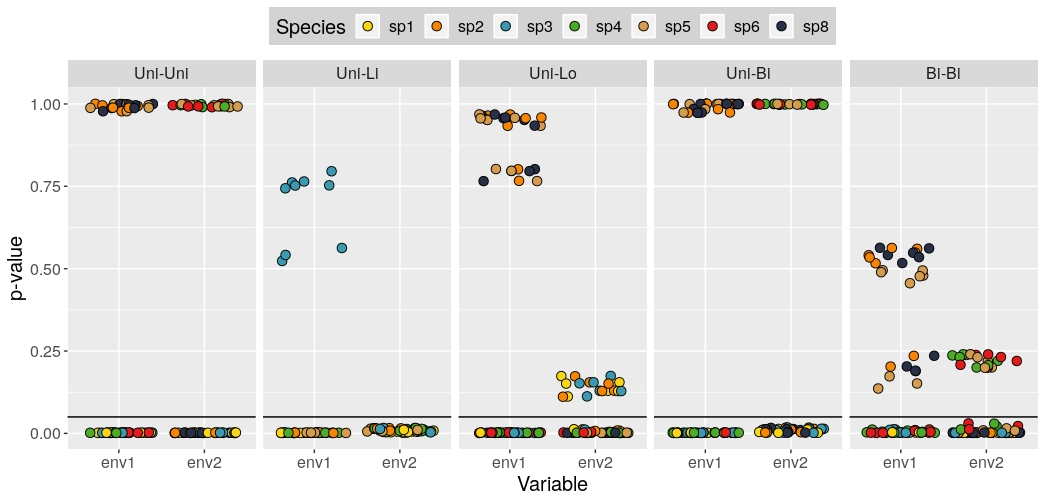
\includegraphics[width=0.9\linewidth]{../02_Figures/01_GLMmv/glm_uni_hohep}
			\caption{
				Univariate GLM$_{mv}$ \textit{p}-values of models containing unimodal or bimodal response types, except \textit{Lo-Bi} and \textit{Li-Bi}. Species that have their optimum at the center of a gradient show higher \textit{p}-values on the corresponding variable. 
				The black line indicates a \textit{p}-value of 0.05. Species identity is indicated via point color.
				Species 7 and 9 are not shown, as their \textit{p}-values did not show any pattern.
				}
			\label{fig:hohep}
		\end{figure}


	%------------------------------%
	%& 	db-RDA 	
	%------------------------------% 
	\subsection{Distance Based Redundancy Analysis}

		db-RDA assigned low \textit{p}-values to most environmental variables.
		%
		Environmental variables only received high \textit{p}-values in \textit{Uni-Li} and \textit{Uni-Lo}, where higher \textit{p}-values were associated with the non-unimodal gradient and class four models.
		%
		For both environmental variables mean \textit{p}-values and standard deviations were highest in class four models. 
		%
		The lowest mean \textit{p}-values for noise variables occurred in \textit{Lo-Lo} at $0.383\ \pm\ 0.206$. 
		%
		\textit{Bi-Bi} had the most noise variable \textit{p}-values below 0.05 and was the only model including one in a class one model. 
		%
		Class three models had the lowest mean \textit{p}-value for noise variables ($Mean\ \pm\ SD\ \scriptscriptstyle Noise,\ class\ 3 \textstyle = 0.431\ \pm\ 0.238$) and class four the highest ($Mean\ \pm\ SD\ \scriptscriptstyle Noise,\ class\ 4  \textstyle = 0.506\ \pm\ 0.289$).\\
		%
		Mean \textit{p}-values for the first constrained axis were low, while for the second they were higher and more spread. 
		%
		For all response types and model classes, environmental variables load stronger on the first two constrained axes than the noise variables.
		%
		The third and higher constrained axes were mostly structured by noise variables and had high \textit{p}-values. 
		%
		The second axis had higher \textit{p}-values in class four models ($Mean\ \pm\ SD\ \scriptscriptstyle CAP2,\ Class\ 4 \textstyle = 0.240\ \pm\ 0.288$)
		than in the other classes ($Mean\ \pm\ SD\ \scriptscriptstyle CAP2,\ Class\ 1,2,3 \textstyle = 0.003\ \pm\ 0.002$).
		%
		This effect is strongest in models with linear or logistic responses.
		%

		%------------------------------%
		%& 	Plot 4: CCA vs. db-RDA p-values 	
		%------------------------------% 
		
		% TODO Graif anders erwähnen
		%Figure \ref{fig:p-compare} shows the \textit{p}-values for \textit{env1} and \textit{env2} as well as the  noise-variables from all models of db-RDA and CCA.
	
	% Figure CCA vs db-RDA p-values.
		\begin{figure}[h!]
			\centering
			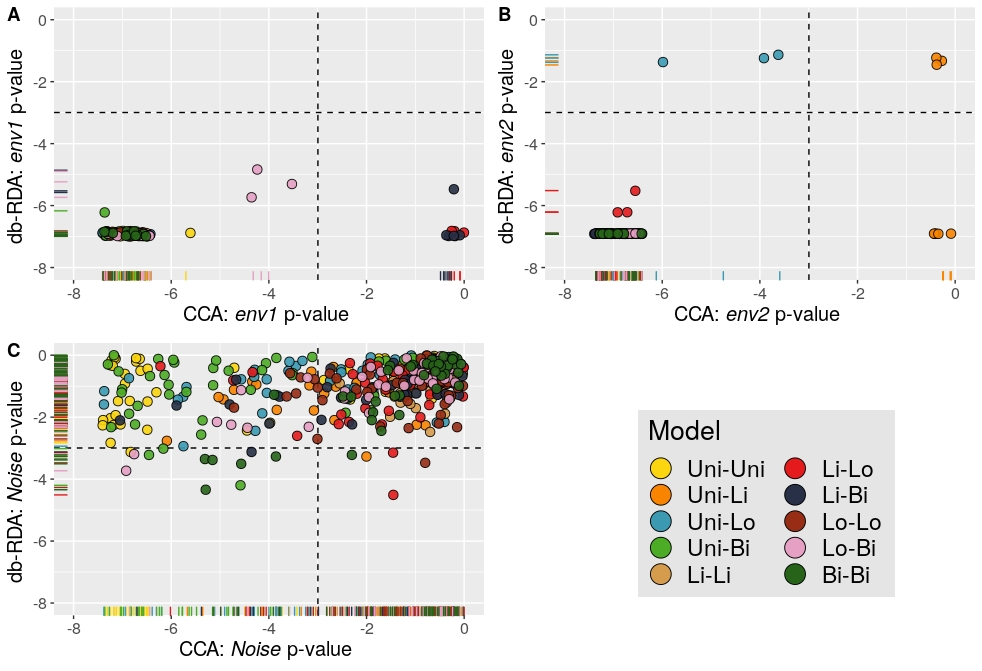
\includegraphics[width=1\linewidth]{../02_Figures/P-Compare}
			\caption{
				\textit{p}-values of (\textbf{a}) \textit{env1},   (\textbf{b}) \textit{env2} and (\textbf{c}) \textit{noise variables} for db-RDA and CCA. Y- and X-axis are scaled with a natural logarithm. Black lines indicated \textit{p}-values of 0.05. Rugs and points are jittered. The color of the points corresponds to the response type combination. 
			}
			\label{fig:p-compare}
		\end{figure}

	%------------------------------%
	%& 			CCA					
	%------------------------------% 

	\subsection{Canonical Correspondence Analysis}

		%------------------------------%
		%& 			Variablen			
		%------------------------------% 
		CCA assigned high \textit{p}-values to linear gradients if only one of the gradients was linear.
		%
		In \textit{Li-Li}, both gradients received low \textit{p}-values.
		%
		Accordingly, mean \textit{p}-values for \textit{env1} and \textit{env2} are high and wide spread. 
		%
		The \textit{p}-values for noise variables were low in comparison to the other methods.
		%
		Leaving out the three models with one linear response (\textit{Uni-Li}, \textit{Li-Lo} and \textit{Li-Bi}), decreased \textit{p}-values of \textit{env1} and \textit{env2} $(Mean\ \pm\ SD\ \scriptscriptstyle env1\ \&\  env2\ \textstyle = 0.001\ \pm\ 0.003$), while the mean \textit{p}-value for noise variables remained at 0.34 $\pm$ 0.32.\\
		%
		Noise \textit{p}-values were especially low in \textit{Uni-Uni} ($Mean\ \pm\ SD = 0.155 \pm\ 0.251$) and \textit{Uni-Bi} ($Mean\ \pm\ SD = 0.118\ \pm\ 0.193$). 
		%
		Noise variable \textit{p}-values in \textit{Bi-Bi} were markedly higher ($Mean\ \pm\ SD = 0.507\ \pm\ 0.336$). \\
		%
		The different classes did not have an impact on \textit{env1} and \textit{env2}. 
		%
		In noise variables the \textit{p}-value decreased when additional noise variables were added and increased with increasing sample sizes. \\
	
		%------------------------------%
		%& 			Axes			
		%------------------------------% 
		The first CCA axis had very low \textit{p}-values, independent of response type or class ($Mean\ \pm\ SD\ \scriptscriptstyle CCA1 \textstyle < 0.001\ \pm\ 0$). 
		%
		For the response combinations \textit{Uni-Li}, \textit{Li-Lo} and \textit{Li-Bi} the second axis had high \textit{p}-values ($Mean\ \pm\ SD\ =  0.459\ \pm\ 0.336$), but was also strongly determined by noise variables.
		%
		Overall, the mean \textit{p}-value for the second axis was higher than for the first.
		%
		Removing the three models \textit{Uni-Li, Li-Lo} and \textit{Li-Bi} reduced its \textit{p}-value to 0.011 $\pm$ 0.055. 
		%
		In \textit{Lo-Bi}, the second axis had considerably higher \textit{p}-values in the class four models 
		($Mean\ \pm\ SD\ \scriptscriptstyle Lo-Bi,\ class 4 \textstyle = 0.260\ \pm\ 0.170$)
		than in the other three classes  
		($Mean\ \pm\ SD\ \scriptscriptstyle Lo-Bi,\ class\ 1,2,3 \textstyle = 0.001\ \pm\ < 0.001$). 
		%
		In all response types, the axes three and higher were determined strongest by noise variables and \textit{p}-values were high. 
		%
		\textit{Uni-Uni} and \textit{Uni-Bi} had low \textit{p}-values for the third and higher axes: 
		$Mean\ \pm\ SD\ \scriptscriptstyle CCA3+, Uni-Uni \textstyle = 0.364\ \pm\ 0.416$;
		$Mean\ \pm\ SD\ \scriptscriptstyle CCA3+, Uni-Bi  \textstyle = 0.407\ \pm\ 0.407$.\\
		
		%------------------------------%
		%& 			Inertia				
		%------------------------------% 
		
		Total inertia differed between response types: Uni- and bimodal responses had the highest total inertia ($Mean\ \pm\ SD\ \scriptscriptstyle Uni/Bi-X \textstyle = 4.45\ \pm\ 1.94$), linear and logistic the lowest ($Mean\ \pm\ SD\ \scriptscriptstyle Li/Lo-X \textstyle = 0.15\ \pm\ 0.13$). 
		%
		Mixtures of these response types lay in between ($Mean\ \pm\ SD\ \scriptscriptstyle Li/Lo-Uni/Bi\textstyle = 1.60\ \pm\ 0.80$).
		%
		This pattern was also found in constrained and unconstrained inertia (see Supplementary Materials Table \ref{tab:ccasm2}).

	%------------------------------%
	%& 			CAO/ CQO			
	%------------------------------% 
	
	\subsection{Constrained Additive and Quadratic Ordination}
	
	%------------------------------%
	%& 	Parameter estimation		
	%------------------------------% 	
	
		For	models with only linear or logistic responses, i.e. \textit{Li-Li, Li-Lo} and \textit{Lo-Lo}, CAO failed to estimate any species parameters. 
		%
		Its also in these models and in \textit{Bi-Bi}, that both variables contributed equally to the latent variable. 
		%
		In the others, one variable determined the latent gradient while the other contributed as much as the noise variables (see Figure \ref{fig:caoonlyone}). 
		%
		\textit{Uni-Lo} was the only response combination for which all parameters were estimated in all classes. 
		%
		In all other combinations, CAO failed to estimate at least some parameters.
		%
		In \textit{Uni-Bi} and \textit{Uni-Uni} estimation failed only for class four models.
		
	%------------------------------%
	%& 	Species Maxima				
	%------------------------------%	
		Species maxima were underestimated for every response combination. 
		%
		The mean difference between estimated and actual maxima, expressed in percent of actual maxima was $-84.9\ \%\ \pm\ 9.3$ \%.\\ 
	
	%------------------------------%
	%& 	Figure: CAO loadings		
	%------------------------------%	
	\begin{figure}[h!]
		\centering
		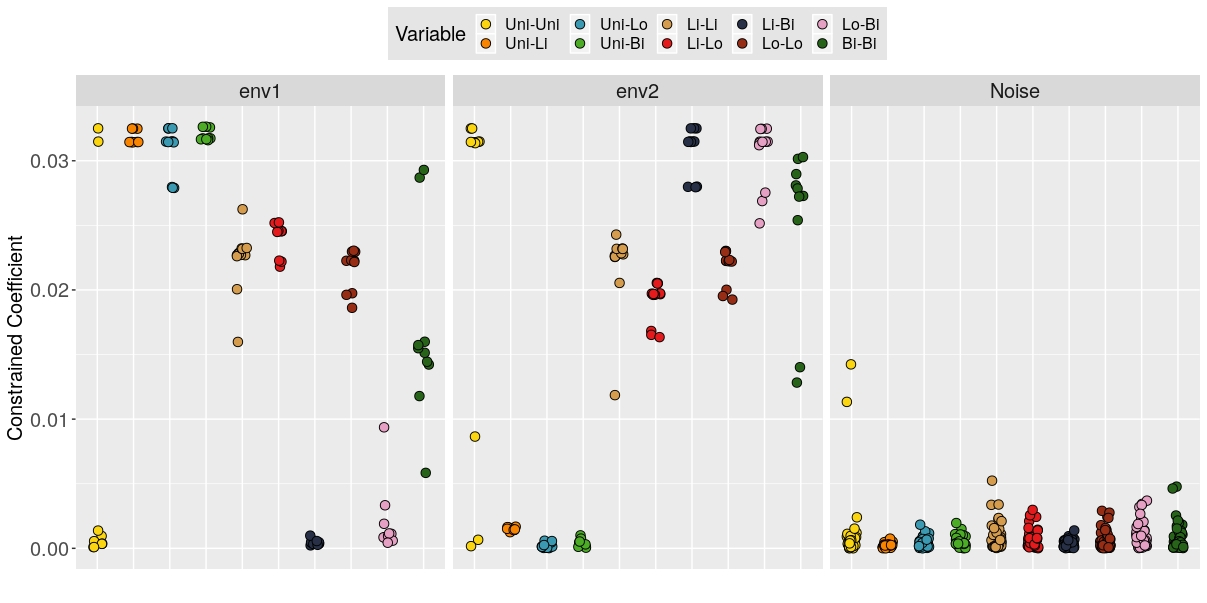
\includegraphics[width=1\linewidth]{../02_Figures/02_CAO/CAO_loadings}
		\caption{
			Absolute values of constrained coefficients from the Constrained Additive Ordination. 
			%
			Colors indicate the response type combination. 
			%
			Each box contains the values for one covariable. 
			%
			Points are horizontally jittered.
		}
		\label{fig:caoonlyone}
	\end{figure}
	%


	%------------------------------%
	%& 			CQO					
	%------------------------------%
	
	Constrained coefficients did not differ significantly between tolerance types, but varied strongly among response types (see Figure \ref{fig:cqoweights}).
	%
	The weights of uni- or bimodal responses were higher than those of logistic or linear ones. 
	%
	The bimodal gradient in class four, unequal tolerance \textit{Li-Bi} (0.277) had the highest coefficient and the linear gradient in the same model the lowest (0.001).
	%
	The weight of a gradient depended not only on the response type but also on the other gradient.
	%
	For example, the mean coefficient of the unimodal gradient in \textit{Uni-Uni} is 0.18, while it is 0.09 in \textit{Uni-Li}. 
	%
	The mean weights for \textit{env1} and \textit{env2} were $0.079\ \pm\ 0.062$ and $0.064\ \pm\ 0.049$. 
	%
	Outliers are often results of class four models, for example, in \textit{Uni-Uni} and \textit{Li-Bi}. 
	%
	However, in some models (e.g. \textit{Uni-Bi}) outliers were generated by other model classes. 

	Overall, the weights of noise variables were markedly lower than those of environmental variables ($Mean\ \pm\ SD_{\scriptscriptstyle Noise} = 0.002\ \pm\ 0.003$).  
	%
	The coefficient was highest in \textit{Uni-Uni} with 0.006 and lowest in \textit{Lo-Lo} with 0.001.
	%
	More noise variables and fewer samples increased the weights of noise variables and decreased those of environmental variables. 
	%
	Additional samples had the opposite effect. \\
	
	There was no overarching effect of either class or tolerance assumption on constrained coefficients. 
	%
	The only notable effect was the lower convergence rate of unequal tolerance models.
	%
	The estimated maxima were extremely inaccurate. 
	%
	In most cases, they were too high, but occasionally also too small. 
	%
	An illustrative example is the equal tolerance, class three, \textit{Uni-Bi} model: For two seeds the maximum abundance of species 9 was overestimated by 1.7e+98 \% of the actual maximum and for the other seed it was underestimated by 100 \%. 
	
	\begin{figure}[h!]
		\centering
		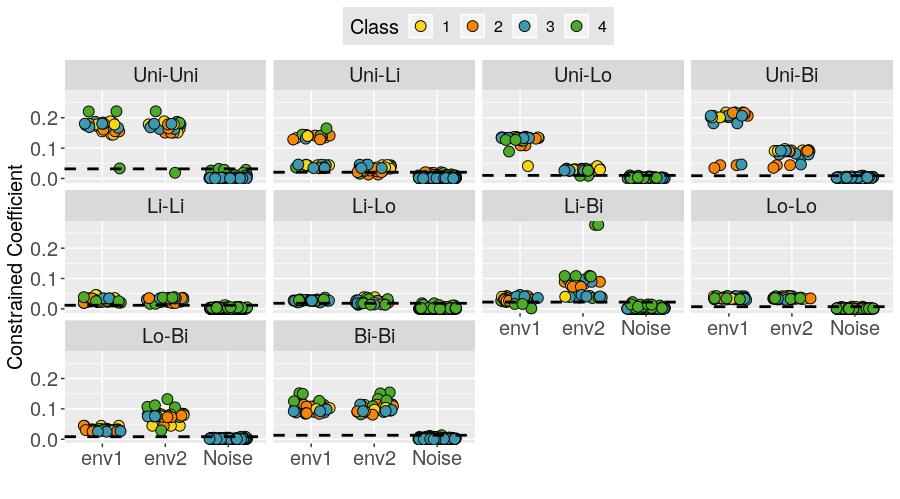
\includegraphics[width=1\linewidth]{../02_Figures/02_CAO/CQOPlotalsJpg}
		\caption{Constrained Coefficients of explanatory variables in a Constrained Quadratic Ordination. Each box is one response type combination. Point colors indicate the model class. The black line marks the highest weight of a noise variable for that response type combination. The points are horizontally jittered. }
		\label{fig:cqoweights}
	\end{figure}
















	
	% !TeX spellcheck = en_US

\section{Discussion}


%------------------------------%
%& 		Repeat what I did		
%------------------------------%
	I ran four different statistical methods (GLM$_{mv}$, db-RDA, CCA, CAO/CQO) on a total of 120 simulated abundance datasets, that differed in response types, sample sizes, number of noise variables and random number generation seeds, to assess their ability to differentiate between environmental variables and noise variables. \\

%------------------------------%
%& 	Ein Satz Fazit für Alle		
%------------------------------%

	The GLM$_{mv}$ correctly assigned low multivariate \textit{p}-values to all environmental variables, and higher ones to noise variables.
	%
	Univariate significance tests also performed well, except for uni- or bimodal gradients receiving high \textit{p}-values for species with optima close to their centers.   
	%
	For class four models GLM$_{mv}$s did not converge.
	%
	db-RDA also differentiated well between environmental and noise variables for all response type combinations.
	%
	However, low sample sizes increased \textit{p}-values for environmental variables and decreased those of noise variables.
	%
	In CCA, linear gradients got high \textit{p}-values if combined with other response types and noise variables had the lowest \textit{p}-values out of all methods used. 
	%
	CAO and CQO showed convergence problems, especially in unequal tolerance CQOs. 
	%
	CAO only estimated all parameters in one of the models (\textit{Uni-Lo}) and failed to estimate any parameters in all models with only linear and logistic gradients.
	%
	As was to be expected, CQO performed best with uni- and bimodal gradients. 
	%
	The constrained coefficient of linear and logistic gradients were frequently  at the level of noise variables.\\


%------------------------------%
%& 			GLMmv				
%------------------------------%

% TODO Viele p-werte unter 0.05 in 15x15 uni 

	GLM$_{mv}$s were least influenced by different response types. 
	%
	They were, however, affected strongest by low sample sizes, as all class four models failed to converge.
	%
	The lowest multivariate \textit{p}-values for noise variables occurred in models that violated the random residuals assumptions (\textit{Li-Bi} and \textit{Lo-Lo}) and thus would likely not be regarded as reliable.
	%
	Species have high univariate \textit{p}-values for a gradient if they reach their optimum near or at the middle of the gradient's sampled range.
	% 
	This is caused by low estimated regression coefficients, which is likely due to the symmetrical nature of the response (see Response Symmetry in GLMs in the Supplementary Materials).
	%
	As it is highly unlikely to observe perfectly symmetrical response shapes right at the middle of the sampled gradient range, it is fair to assume that these problems were due to the simulation set up and improbable in field data.  
	%
	Another problem of GLM$_{mv}$ is the long runtime, which is due to the resampling \citep{Wang2012}.
	%
	%
	By resampling, one avoids having to specify the correlation between species in the model.
	%
	The correlation is accounted for at the inference stage by resampling observations across independent sites \citep{anderson2001new}. 
	%
	Models that include the correlation structure explicitly avoid resampling and thus can reduce computation time.
	%
	First advances in this direction have been made, e.g. by \citet{Jamil2012} who used the site effect of a Generalized Linear Mixed Model (GLMM) to induce equal correlation between all species pairs.\\
	%
	In contrast to the other considered methods, GLM$_{mv}$s do not reduce the dimensions of the data. 
	%
	Visualizing the multivariate and thus multidimensional data is therefore cumbersome.
	%
	Indeed, no easy-to-use and to interpret method to present the output of GLM$_{mv}$s is available. \\
	%
	Many features of GLM$_{mv}$s remain unexplored in this study. 
	%
	I only tested the model under the assumption of independence of species.
	%
	Other correlation type settings can account for dependence between species, either with an unstructured correlation matrix (only advisable when $N>S$) or by shrinking the correlation matrix towards identity using ridge regularization \citep{warton2008penalized}.
	%  
	These correlation types necessitate the usage of another test statistic than the likelihood ratio. 
	% 
	Currently, the Wald test statistic and the score statistic are also implemented to this end.
	% 
	The Wald test statistic makes use of GEE with the sandwich-type-estimator of \citet{Warton2011a} but is unsuitable for count or occurrence data with means at zero. 
	%
	For such cases, the score statistic should be used. 
	%
	Datasets simulated to test these variants of GLM$_{mv}$ could highlight performance differences even more strongly, as the other methods do not incorporate adjustments to these properties. \\

%------------------------------%
%& 		db-RDA		
%------------------------------%

	db-RDA also proved to be robust to different response types and sample sizes. 
	%
	Although, low samples sizes decreased the method's power in \textit{Uni-Lo} and \textit{Uni-Li}. 
	%
	The six models with high \textit{env2} \textit{p}-values (cf. Figure \ref{fig:p-compare}) are all class four models.
	%  
	db-RDA's good performance is in concert with other simulation studies \citep[e.g.][]{Roberts2009}.
	%
	Hence, its popularity in the ecological community seems justified. 
	%
	These results are only valid for the Bray-Curtis Distance metric, which was used here.
	%  
	Other measures would likely have produced different results, 
	therefore the selection of an appropriate metric is a crucial step in any db-RDA analysis.
	%  
	Having to choose a single metric can be avoided by using consensus RDA \citep{Blanchet2014}.
	% 
	In this novel method, multiple db-RDA are run, only differing in their distance metric. 
	%
	Site scores on statistically significant axes are combined into one matrix which acts as response matrix in a new RDA. 
	%
	This method extracts the information that is common to all individual models.
	%
	Simulation studies comparing properties of consensus RDA with those individual db-RDA and other methods, distance- or model-based, are lacking.
	% 
	Another avenue for future development of db-RDA would be novel distance metrics, but there have been no recent developments (M. J.Anderson, pers. comm.).\\

%------------------------------%
%& 				CCA				
%------------------------------%

	The CCA performed worst of the methods tested. 
	%
	Linear responses were categorically assigned high \textit{p}-values if they were combined with other response types. 
	%
	The method should thus not be used for combinations of linear and non-linear responses.
	%
	Linear response usually occur if the sampled gradient is short relative to the species' tolerance. 
	%
	For axes as well as terms the noise \textit{p}-values were lower than in other methods.
	% 
	Most low \textit{p}-values for noise variables in CCA occurred in uni- or bimodal models. 
	%
	Given that \textit{Uni-Uni} fits the expectations of the species packing model and bimodal models do not deviate strongly (responses are symmetric but not bell-shaped), this is surprising.
	%
	These models also had higher inertia than those with linear or logistic gradients, which suggests that the type-I-error rate might be related to the inertia (see Supplementary Materials Table \ref{tab:smcca5} and \ref{tab:smcca6}). 
	%
	Given that the triplots (see Supplementary Materials Figure \ref{fig:smccaord}) are not skewed by noise variables with low \textit{p}-values, the problem might also reside in the method that is used to calculate the \textit{p}-values. \\
	%
	%The low total inertia in models with linear gradients might be the reason that CCA assigned high \textit{p}-values to these gradient and axes that were determined by them.
	%%
	%Even if the ratio of constrained to total inertia is higher in the linear gradient, the non-linear one will always introduce more total inertia and therefore in absolute terms also more constrained inertia to the CCA. \\
	%
	Newer approaches to CCA that can correct for zero inflation \citep{Zhang2012} or non-linear relationships between predictor and response variable \citep{Makarenkov2002} are available but not widely used.  \citet{TerBraak2015} advocate to move beyond Gaussian Ordination and further develop methods that are based on smooth functions, like the CAO. \\

%------------------------------%
%& 			CAO					
%------------------------------%
	%In this study CAO was mainly used as a exploratory method as suggest by \citet{Yee2006}.
%
	%Nevertheless, it is instructive to regard its results in their own rights. 
%
	In CAO, estimation of optima and maxima failed in all models that only included linear and logistic responses.
	%
	In most other models, estimates for some species were missing, particularly those with optima close to the end of the sampling range. 
	%
	Species maxima were underestimated in all response type combinations.
	%
	This was strongest in \textit{Uni-Uni} and \textit{Uni-Bi}, which adhere the closest to the assumptions of CQO.\\ 
	%
	In most models, only one gradient significantly influenced the latent variable (see Figure \ref{fig:caoonlyone}), even if both gradients were identical (e.g. \textit{Uni-Uni}). 
	%
	This problem might improve with rank-2 CAOs but further tests, also with more than two environmental variables, are necessary.  
	%
	Using a CAO to test for unimodality and thus whether to use or to discard a variable for a CQO was rather conservative for these data.
	%
	Parameter estimation even failed for some species in \textit{Uni-Uni} and \textit{Uni-Bi}. 
	%
	\citet{Jamil2013} present an alternative, graphical tool based on GLMMs to test for unimodality, which was applied by \citet{jamil2014unimodal}, though not in connection with CQO. 
	%
	Overall, the CAO was no reliable guide CQO-suitability and estimated species parameters systematically diverged from the actual values. 
	%
	However, many features of this method, e.g. rank-2 models and further residual distributions, are not yet implemented in VGAM  \citep{yee2015vector}.
	%
	Alternative methods using smooth functions for ordination are also available \citep[e.g.][]{schnabel2012modeling}\\

%------------------------------%
%& 			CQO					
%------------------------------%

	The weight that CQO assigned to different response types varied strongly.
	%
	The mean weight of environmental gradients was always higher than that of noise variables, but some individual linear or logistic gradients have constrained coefficients on the level of noise variables.  
	%
	Uni- and bimodal gradients had higher weights than linear or logistic ones. 
	%
	However, the response types also influenced each other. 
	%
	The weight of uni- or bimodal gradients was much lower when combined with linear or logistic gradients instead of each other.
	%
	How the influence of gradient types on each others constrained coefficient develops in settings with more than just two variables, as one would expect in actual communities, would be an interesting avenue for further studies. \\
	%
	The impact of different numbers of samples and noise variables was, besides the convergence problems with some class four models, negligible.
	%  
	The same holds true for different tolerance settings. 
	%
	The most notable difference was the lower convergence rate in unequal tolerance models.
	%
	Equal tolerance models ran longer than those with unequal and identity tolerance. 
	%
	Since tolerances have to be estimated individually in unequal tolerance models these were expected to run the longest \citep{yee2015vector}.  
	%
	The estimates for abundance maxima were very inaccurate and mostly too high. Based on the strength of divergence between estimated and real values, I advise against using these maxima.\\
	%  %Baselga & Araújo 2009 finde ich nicht mehr 
	Up until now, usage of CQO and CAO is seldom in ecological studies and mostly within fisheries research (e.g. \citet{Vilizzi2012}, \citet{Top2016} and \citet{Carosi2017}). 
	% 
	\citet{TerBraak2015} suggest that this is due to limitations on the number of species that can be included, a steep learning curve and numerical instability. 
	%
	This study confirmed that in its current state the method has issues with convergence and parameter estimations. 
	%
	It is especially concerning that the weights of unimodal gradients can be decreased by other non-unimodal gradients and that estimated maxima are overestimated. \\ 

%------------------------------%
%& 		Simulated Data			
%------------------------------% 

	Further steps can be taken, to render the simulated data more alike actual field data. 
	%
	\citet{Austin1999} criticized unimodal and symmetric response curves as overly simplistic and \citet{austin1994determining} proposed beta-functions to simulate unimodal but asymmetrical shapes. 
	%
	However, in a study of \citet{Oksanen2002} only about 20\% of the responses were strongly skewed, while symmetric and bell shaped responses were the most common. 
	%
	In this study, I opted to use bimodal and logistic responses as skewed versions of the bell-shape instead of beta functions. \\
	%
	Also, species abundances were only determined by the environmental gradients. 
	%
	Stochasticity can be added to one or to both ends of the relationship. 
	%
	For example, in form of a random term, which is added to the abundances or environmental variables \citep[e.g][]{McCune1997}.
	%
	Likewise, observation errors can be included via binomial functions, as is done in N-mixture models \citep{royle2004n},
	to examine how susceptible a method is towards regression dilution \citep[e.g.][]{frost2000correcting, McInerny2011}.
	%
	Lastly, when noise is added to response and explanatory variables this would, given the noise is simulated from the same distribution both times, likely result in endogeneity, i.e. a non-zero covariance between the residuals and one or more explanatory variables. 
	%
	Simulations with induced endogeneity would be interesting as this phenomenon might be underappreciated by ecologists \citep{armsworth2009contrasting, fox2015ecological}. \\ 

% ---------------------------------------- %
%&		Andere Vergleichende Studien		
% ---------------------------------------- %
 
 	The methods that were compared in this study have never been directly compared before. 
 	%
 	Most similar is the work of \citet{Warton2012}, who compare GLM$_{mv}$ to CCA and RDA (not db-RDA) among others. 
 	%
 	They showed that only GLM$_{mv}$ successfully differentiates between location effect (difference in means) and dispersion effect (difference in variance). 
 	%
 	However, comparative studies of multivariate methods, in general, are common. 
 	%
 	Especially ordination techniques like CCA and RDA were subject to extensive testing in the 1970s and 1980s \citep[e.g.][]{GauchJr.1972, GauchJr1977, Kenkel1986}. 
 	%
 	To my knowledge, \citet{Roberts2008} and \citet{Roberts2009} are the only studies that methodically compare db-RDA to other methods. 
 	%
 	Both compare db-RDA, CCA and Multidimensional Fuzzy Set Ordinations (MFSO). \citet{Roberts2008} uses simulated data sets to this end, while \citet{Roberts2009} uses four different sets of field data. 
 	%
 	Both studies concur that db-RDA outperforms CCA and is tied with or performs slightly inferior to MFSO. 
 	%
 	CQO/CAO are occasionally tested in comparisons of individual and community level species distribution models (e.g. \citet{Baselga2009} and \citet{Maguire2016}), where they are an instance of the latter.
 	%
 	They were generally not found to significantly improve upon the individual models (e.g. GLMs or Regression Trees). 
 	\\
 
%------------------------------------------------%
%& Andere Vielversprechende Model-based approaches
%------------------------------------------------%

	In this study, one (GLM$_{mv}$) model-based approach outperformed both the distance-based and the algorithmic approach, while the other (CQO) was not clearly superior, at least not to db-RDA.
	%
	Both, GLM$_{mv}$ and db-RDA proved robust towards any response type tested herein, while both having poorer properties with little sample sizes. 
	%
	CCA should not be used for linear responses, i.e. short gradients, and the term \textit{p}-values are very low for noise variables, especially in models with high inertia. 
	%
	The comparison to CAO and CQO is complicated by the absence of a common statistic. 
	%
	Both showed issues with convergence and estimation accuracy. 
	%
	Constrained Coefficients varied strongly between response types and within some models (CAO e.g. \textit{Uni-Uni}, CQO e.g. \textit{Li-Bi}). 
	%
	Even for models with unimodal response type CQO severely overestimated the maximal abundances, this parameter should hence not be used. 
	%
	This study thus showed, that some but not all approaches in model-based multivariate inference have considerable potential and can outperform more common distance-based or algorithmic methods. 
	%
	As these models are still at an early stage, new developments and increases in computation speed can be expected.   
	\\

	% ------------------------- %
	%&		Joint Models		
	% ------------------------- %
	
	An especially active area are models using joint probability distributions \citep[e.g.][]{Clark2014, Pollock2014}. 
	%
	While GLM$_{mv}$ estimate the mean of the conditional distribution $Y_s$   given  $\mathbf{X}$ ($\hat{E}(Y_s|\mathbf{X})$) separately for each species and CQO combine all species to estimate the latent variable but regress each species separately against them,
	joint models estimate the joint distribution of all species conditional on the environmental variables.  
	%
	%\citet{Clark2014} show that basal area of trees is better predicted by joint distribution models than by independently calibrated models. 
	%
	A common interest of many joint models is to imply biotic interactions from the residuals of the species-environment interaction, 
	%
	as these two sets of predictors (biotic and biotic) were shown to have little redundancy \citep{Meier2010}.
	%
	Some of the models also anticipate the challenges of Big Data for ecology \citep{Hampton2013}.
	%
	\textit{Generalized Linear Latent Variable Models}, for example, include latent variables instead of random effects to capture residual correlation, which significantly reduces the size of the variance -- covariance matrix \citep{Warton2015,Niku2017}.  
	%
	In HMSC \citep{Ovaskainen2017} this approach is coupled with a fourth corner model \cite[including species traits, ][]{legendre1997relating} and phylogenetic relationships to make sense of many types of data.
	%
	To the same end, GJAMs allow for different kinds of data (e.g. continuous, discrete counts, ordinal counts and occurrence) to be included in the same response variable and have outperformed Poisson GLM on discrete count data and a Bernoulli GLM on binary host status data in a recent simulation study \citep{Clark2017}. \\
	
	
	It is now essential that ways to infer ecological processes from the modeled patterns develop at a similar pace, to avoid confusing statistical artifacts with genuine biological signals \citep{dormann2018biotic}.
	%
	If this succeeds, a move form distance-based and algorithmic methods towards model-based methods might entail one from the current implicit Gleassonian towards a from of modern Clementsian perspective \citep{Eliot2011}; from asking how do individual species change along environmental gradients towards asking how do communities change as a whole.   


%---
%& GJAM
%---

 
% GJAM (avialable in gjam R package )  allow for different kinds of response data to be modeled for the same species. This includes continuous (e.g. biomass or density), discrete counts, ordinal counts (none, some, many) and incidence (present, absent). They also include the relative measurement effort (e.g. search time for counts or core volume sediment cores), since higher effort is likely to lead to reduced variability. In a simulation study GJAM outperformed Poisson GLM on discrete count data and a Bernoulli GLM on binary host status data \citep{Clark2017}.  


%%% --- Allgemein--- %%%
% - usually gradients are not the measured variables 
% - biotic interaction, succseional or priority effects not considered , changes in species richness along gradients.
% - GLMmv nicht ausgereizt. 



	

	\newpage
		
	\small
	\addcontentsline{toc}{section}{References}	
	
	\bibliographystyle{apalike}

	\bibliography{Bib/Master_Bib}
	%\bibpunct{()}{)}{;}{a}{}{;}
	\newpage
	% !TEX spellcheck = en_US

\section{Supplementary Materials}


	\subsection{Response Symmetry in GLMs}
		\normalsize
		In the univariate significance tests of  GLM$_{mv}$s, species with optima at the middle of an uni- or bimodal gradient were assigned high \textit{p}-values. 
		%
		Here, I will show that this likely occurred due to the symmetry of the response shape when considered over the whole sampling range. 
		%
		Figure \ref{fig:uniglm} shows three unimodal responses that only differ in the position of their optimum. One (orange) is at 50 which is exactly the middle of the sampled gradient, as is indicated by the dashed line, one (blue) is at 49 and the last (green) at 25. 
		
		% ---------------------------------------------------------------------------- %
		%& Figure: Unimodal response shapes and corresponding regression coefficients
		% ---------------------------------------------------------------------------- %
		
		\begin{figure}[h!]
			\centering
			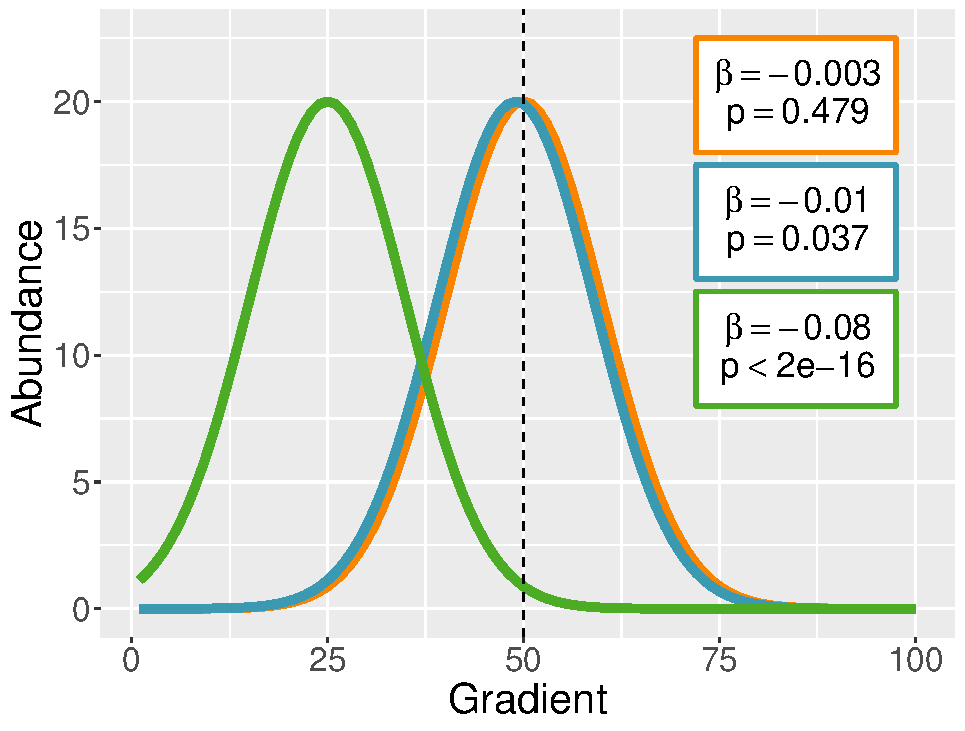
\includegraphics[width=0.5\linewidth]{../02_Figures/uniglm/uniglm}
			\caption{
					Unimodal response shapes with different optima.
					%
					The dashed line indicates the middle of the sampled range.
					%	
					Each color represents a different species.
					%
					The response shapes only differ in the location of their optimum, both tolerance and maximal abundance are equal.
					%
					$\beta$ refers to the regression coefficient for the gradient in a GLM which models abundance as a function of the gradient and p to the corresponding \textit{p}-value.
					%
					The color of the boxes indicates which curve the values belong to.
					%
					The regression coefficient increase and the \textit{p}-values decrease as the distance of the optimum from the middle of the gradient increases.  
					}
			\label{fig:uniglm}
		\end{figure}
		   
		The \textit{p}-values and regression coefficients come from a GLM with negative binomial residual distribution, conducted with the MASS R-package \citep{Venables2002}.
		%
		The small difference in optima between the orange and the blue species entails a big disparity in regression coefficients. 
		%
		The regression coefficient of the blue species is approximately three times higher and the \textit{p}-value is less than a tenth of the orange ones.
		%
		The green species shows that the regression coefficient further increases and the \textit{p}-value further decreases as the optimum is farther removed from the middle. 
		%
		These results were comparable but not identical to those obtained when using optima higher than 50 (not shown here).\\
		
		% ---------------------------------------------------------------------------- %
		%& Figure: Bimodal response shapes and corresponding regression coefficients
		% ---------------------------------------------------------------------------- %
		
		\begin{figure}[h!]
			
			\begin{subfigure}{0.5\textwidth}
				\centering
				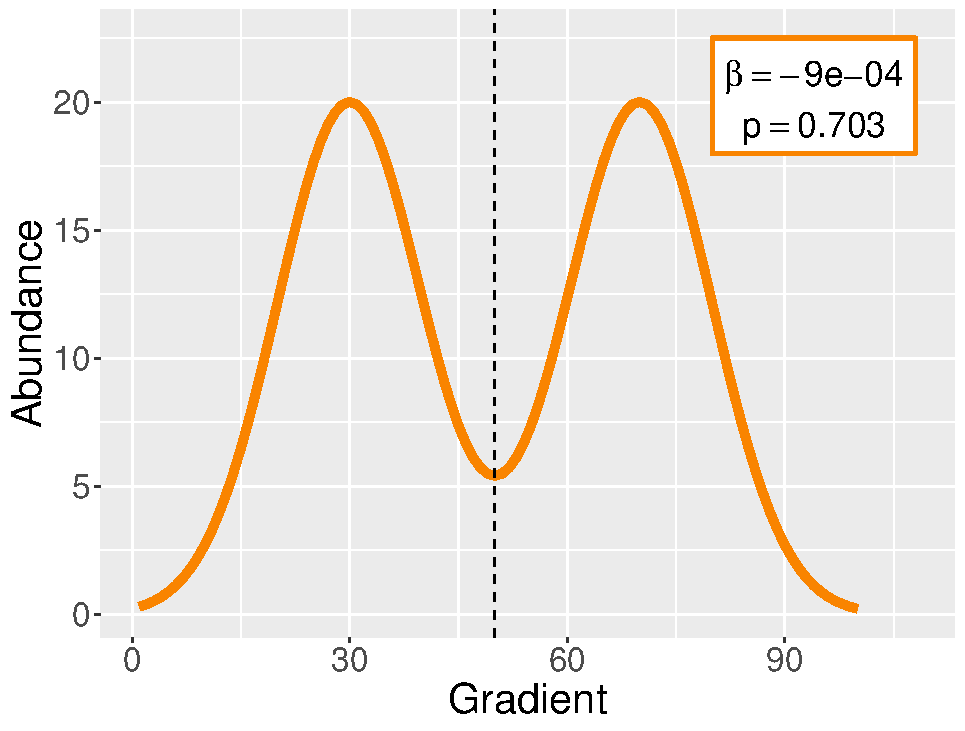
\includegraphics[width=1\linewidth]{../02_Figures/uniglm/bi1}
				\caption{}
				\label{fig:biglm1}
			\end{subfigure}
			\begin{subfigure}{0.5\textwidth}
				\centering
				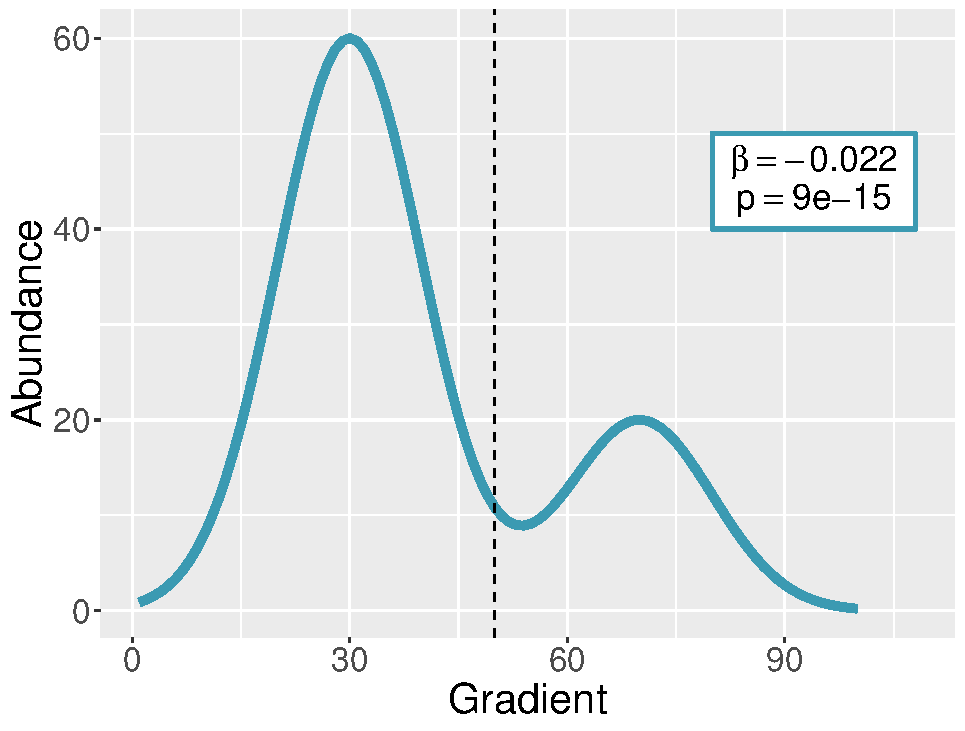
\includegraphics[width=1\linewidth]{../02_Figures/uniglm/bi2}
				\caption{}
				\label{fig:biglm2}
			\end{subfigure}
			\begin{subfigure}{0.5\textwidth}
				\centering
				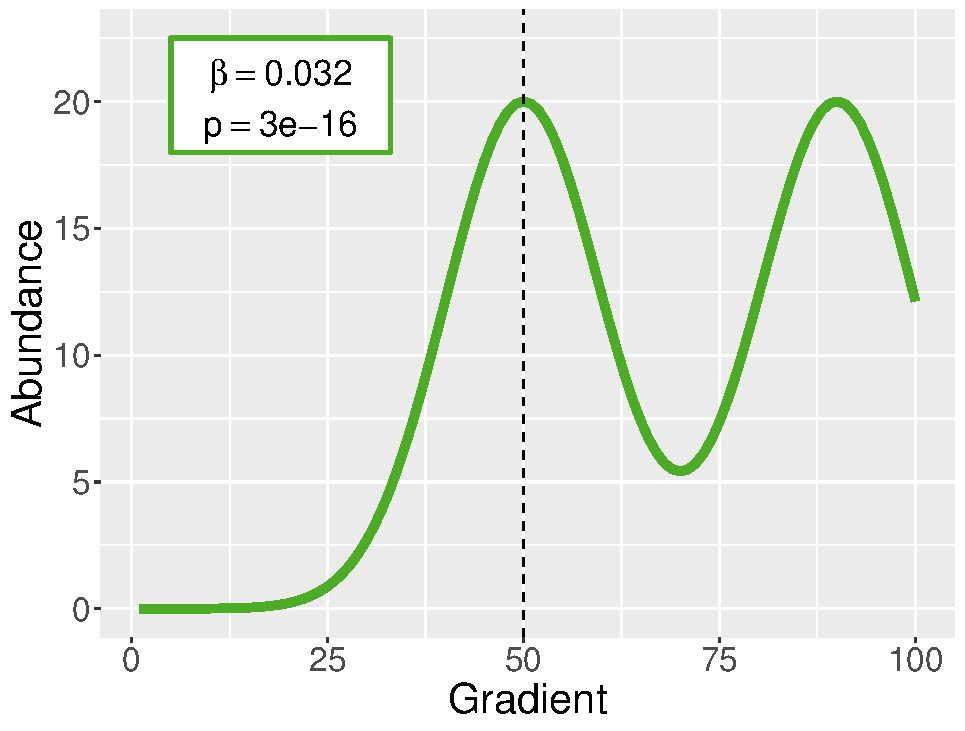
\includegraphics[width=1\linewidth]{../02_Figures/uniglm/bi3}
				\caption{}
				\label{fig:biglm3}
			\end{subfigure}
			\caption{
				Bimodal response shapes. 
				%
				In the boxes $\beta$ is the regression coefficient for the gradient in a GLM which models Abundance as a function of the gradient. 
				%
				p is the associated \textit{p}-value. 
				%
				The dashed line indicates the middle of the sampled range.
				%
				(\textbf{a}) shows a symmetrical response, $\beta$ is low and the \textit{p}-value is high. 
				%
				(\textbf{b}) and (\textbf{c}) are asymmetrical modifications of (\textbf{a}). 
				%
				In (\textbf{b}) the maximum of the first optimum is higher than the second. 
				%
				This results in a higher $\beta$ and lower \textit{p}-value. 
				%
				(\textbf{c}) shows the same response shape as (\textbf{a}) but shifted to the right. 
				%
				This modification also results in a higher $\beta$ and lower \textit{p}-value.
			}
			\label{fig:biglm}
		\end{figure}
		
		
		Figure \ref{fig:biglm} shows a similar setup for bimodal response shapes. In figure \ref{fig:biglm1} the response is symmetrical. 
		%
		The middle of the gradient lies exactly between the two optima.
		%
		A GLM with negative binomial residual distribution returns a low regression coefficient (- 9e-04) and an appropriately high \textit{p}-value (0.703).
		%
		For figure \ref{fig:biglm2}, the maximal abundance at the first optimum was increased to three times that of the second.
		%
		The middle of the response shape still coincides with that of the gradient.
		%
		The regression coefficient (-0.22) is increased (in absolute terms) relative to the first model and the \textit{p}-value (9e-15) is decreased. 
		%
		A similar pattern can be observed when the response shape of figure \ref{fig:biglm1} is shifted to the right, as is done in figure \ref{fig:biglm3}.
		%
		Again, the regression coefficient (0.032) is increased and the \textit{p}-value (3e-16) decreased.\\
		
		These examples show that the symmetry of the response shape over the whole sampling range leads to small regression coefficients and the corresponding high \textit{p}-values. 
		%
		They also demonstrated that already small deviations from this symmetry (1/100 of the gradient length as the blue species in Figure \ref{fig:uniglm}) substantially increases the coefficient and decreases the \textit{p}-value.  
	
		
	
	\subsection{Further Details on Simulations} 
	
		The Table \ref{tab:SimDet} shows the model parameters used in the simulation.
		
		% ------------------------- %
		%& Table: Model parameters 
		% ------------------------- %
		\begin{table*}[h]
			\small
			\centering
			\caption{Model parameters used in simulations. An x indicates that the parameter is not relevant to the gradient types used. \textit{c} is the maximal abundance, \textit{t} the tolerance, \textit{u} the location of the optimum, $x_0$ the midway points of the sigmoid, $\beta$ the  linear response parameter and \textit{k} the steepness of the logistic curve. Values in braces are optima pairs for bimodal gradients.}
			\begin{tabular}{@{}llllll@{}}
				\toprule
				        & \textit{c} & \textit{t} & \textit{u}/ $x_0$                                 & $\beta$                & \textit{k}     \\
				\hline       
				Uni-Uni & 100 & 7.5 & 20, 50, 80                                                & x                   		  & x     \\
				Uni-Li  & 100 & 7.5 & 0, 25, 50, 75, 100                                        & 1, 1.2, 1.4, 1.6, 1.8       & x     \\
				Uni-Lo  & 100 & 7.5 & 20, 50, 80                                                & x                   		  & 0.1 \\
				Uni-Bi  & 100 & 5   & 20, 50, 80/ \{10, 30\}, \{40, 60\}, \{70, 90\}                        & x                  		  & x  \\
				Li-Li   & x   & x   & x                                                         & 80, 100, 120, 0.8, 1.1, 1.2 & x     \\
				Li-Lo   & 100 & x   & 15, 30, 45, 60, 75                                        & 0.1                   	  & 0.05  \\
				Li-Bi   & 100 & 6   & \{5, 25\}, \{25, 45\}, \{35, 55\}, \{55, 75\}, \{75, 95\} & 0.1                    	  & x     \\
				Lo-Lo   & 100 & x   & 20, 50, 80                                                & x                     	  & 0.1   \\
				Lo-Bi   & 100 & 6   & 20, 50, 80/ \{5, 25\}, \{35, 55\}, \{75, 95\}             & x                      	  & 0.1   \\
				Bi-Bi   & 100 & 6   & \{5, 25\}, \{35, 55\}, \{75, 95\}                         & x                      	  & x     \\
				\toprule
			\end{tabular}
			\label{tab:SimDet}
		\end{table*}
		\normalsize	
		The optimum parameter \textit{u} is the only instance of a parameter that is relevant to both gradients and differing between them. 
		%
		The different values are separated by forward slashes. 
		%
		Bimodal gradients require two optima per species. 
		%
		The used combinations are shown in braces. \\
		%
		In \textit{Li-Li}, the first three species reacted to \textit{env1} the next three to \textit{env2} and the last three to both.
		%
		For this reason, the $\beta$ parameters of the last three species are much lower than the first three. 
		%
		This also causes the high \textit{p}-values for \textit{env1} and \textit{env2} in \textit{Li-Li} (see Table \ref{tab:GLMUNI1}). 
		
	\subsection{Ordination Diagrams}
	
		As the result of dimension reduction, db-RDA, CCA, and CAO/CQO produce ordination diagrams. 
		%
		In the following section, a selection of diagrams will be presented for all four methods. \\ 
		%
		This selection will include the models: \textit{Uni-Uni}, \textit{Uni-Li}, \textit{Li-Li} and \textit{Lo-Lo}.
		%
		The first diagrams are from the db-RDA analyses (Figure \ref{fig:smdbord}). 
		%
		All subplots include explanatory variables (blue arrows), species scores (red letters), site scores as linear combinations of explanatory variables (grey points, LC-scores) and sites scores as weighted averages of species scores (green triangles, WA-scores).
		%
		These data are plotted in scaling 1 (distance-triplot) and can be interpreted as follows: 
		%
		i.) the angles between explanatory variables and the arrow that could be drawn from the centroid to each species score represent their correlation, %
		ii.) distances between objects approximate their Euclidean distance.\\
		%
		The species scores are positioned correctly in Figure \ref{fig:smdbord} a-c but in d the original pattern is not recognizable anymore. 
		%
		LC-scores always form  squares and the distance between the points is approximately constant. 
		%
		WA-scores are more prone to deformation. 
		%
		In \ref{fig:smdbord} a WA-scores are concentrated around species scores, in b they are fan-shaped, in c they look good and in d they appear to form a circle instead of a square.
		%
		In all models explanatory variables either load equally strong on both axes or each load on a separate axis.
	
		% ----------------------------------- %
		%& Figure: db-RDA ordination diagrams 
		% ----------------------------------- %
		\begin{figure}[h!]
			
			\begin{subfigure}{0.5\textwidth}		
					\centering
					\includegraphics[width=.55\linewidth]{"../02_Figures/04_dbRDA/01_LLGB/Triplots/Use in SM/17_S1_plot1"}
					\caption{Uni-Uni}
			\end{subfigure}
			%
			\begin{subfigure}{0.5\textwidth}
					\centering		
					\includegraphics[width=.55\linewidth]{"../02_Figures/04_dbRDA/01_LLGB/Triplots/Use in SM/21_S1_plot1"}
					\caption{Uni-Li}
			\end{subfigure}
			%
			\begin{subfigure}{0.5\textwidth}	
					\centering	
					\includegraphics[width=.55\linewidth]{"../02_Figures/04_dbRDA/01_LLGB/Triplots/Use in SM/33_S1_plot1"}
					\caption{Li-Li}
			\end{subfigure}
			\begin{subfigure}{0.5\textwidth}		
					\centering
					\includegraphics[width=.55\linewidth]{"../02_Figures/04_dbRDA/01_LLGB/Triplots/Use in SM/45_S1_plot1"}
					\caption{Lo-Lo}
			\end{subfigure}
			
			\caption{Triplots of the db-RDA analyses of (\textbf{a}) Uni-Uni, (\textbf{b)} Uni-Li, (\textbf{c}) Li-Li and (\textbf{d}) Lo-Lo. For every response combination the class 1 model was used.}
			\label{fig:smdbord}
			
		\end{figure}
	
		%& CCA
		
		Figure \ref{fig:smccaord} shows the triplots of the CCA analyses.
		%
		The same symbology as in Figure \ref{fig:smdbord} was used.
		%
		Again, scaling 1 is utilized.
		%
		In CCA this can be interpreted following these rules: 
		%
		i.) An orthogonal projection from an object (site or species score) on an explanatory variable approximates that object's position along that variable, ii.)  distances among object approximate their chi-squared distance. \\
		%
		In Figure \ref{fig:smccaord} a,c and d the species scores are placed correctly relative to the explanatory variables. 
		%
		In \textit{Uni-Li} they are only ordered along the unimodal gradient and the second axis is determined by noise variables.
		%
		The LC-scores form are square and are equidistant in \textit{Uni-Uni} and \textit{Lo-Lo}. 
		%
		In \textit{Uni-Li} they appear to be randomly distributed and in \textit{Li-Li} they are fan-shaped with the distance between points increasing towards lower values of the explanatory variables. 
		% 
		WA-scores are concentrated around species scores in \textit{Uni-Uni}, fan-shaped in \textit{Li-Li} and \textit{Lo-Lo} and scattered, though mostly absent in \textit{Uni-Li}. 
		In contrast to the db-RDA triplots, the species scores never lie outside the site scores. 
		
		% ----------------------------------- %
		%& Figure: CCA ordination diagrams 	
		% ----------------------------------- %		
		\begin{figure}[h]
			\begin{subfigure}{0.5\textwidth}		
				\centering
				\includegraphics[width=.8\linewidth]{"../02_Figures/03_CCA/01_LLGB/Triplots/use in SM/17_S1_plot1"}
				\caption{Uni-Uni}
			\end{subfigure}
			%
			\begin{subfigure}{0.5\textwidth}
				\centering		
				\includegraphics[width=.8\linewidth]{"../02_Figures/03_CCA/01_LLGB/Triplots/use in SM/21_S1_plot1"}
				\caption{Uni-Li}
			\end{subfigure}
			%
			\begin{subfigure}{0.5\textwidth}	
				\centering	
				\includegraphics[width=.8\linewidth]{"../02_Figures/03_CCA/01_LLGB/Triplots/use in SM/33_S1_plot1"}
				\caption{Li-Li}
			\end{subfigure}
			\begin{subfigure}{0.5\textwidth}		
				\centering
				\includegraphics[width=.8\linewidth]{"../02_Figures/03_CCA/01_LLGB/Triplots/use in SM/45_S1_plot1"}
				\caption{Lo-Lo}
			\end{subfigure}
			
			\caption{Triplots of the CCA analyses of (\textbf{a}) Uni-Uni, (\textbf{b)} Uni-Li, (\textbf{c}) Li-Li and (\textbf{d}) Lo-Lo. For every response combination the class 1 model was used.}
			\label{fig:smccaord}
		
		\end{figure}
		\newpage
		Figure \ref{fig:smcaoord} shows the latent variables plots of the CAO analyses. 
		%
		The x-axis shows the value of the latent variable and the y-axis the estimated abundance.
		%
		Each curve represents one species and is identifiable via the labels next to it.
		%
		The plot for \textit{Uni-Uni} in Figure \ref{fig:smcaoord}a depicts the species as belonging to one of three groups based on their optimum.
		%
		Based on the species identities (1, 4, 7 in group 1; 2, 5, 8 in group 2; 3, 6, 9 in group 3) it can be inferred that the latetent variable is only structured along \textit{env1}.
		%
		The species belonging to group 2 have lower maximal abundances than those in group 1 and 3, but all species lie below their actual maxima, which is 1000 for every species.  
		%
		In \textit{Uni-Li} species are only ordered along the unimodal gradient \textit{env1}.
		%
		The abundances of species 1 and 5, which have their optima outside of the sampled range, are markedly higher than those of the other species and also higher than the model maxima.
		%
		These \textit{edge effects} in \textit{Uni-Uni} and \textit{Uni-Li} are common in CAO and CQO. 
		%
		Estimation of species with parts of their response outside the latent variable space failed more often and were the least accurate. \citet{yee2015vector} advises to drop the corresponding species form the analysis.\\
		In \textit{Li-Li} the smoothing induces a slight curve in the response shape, especially in the species 7 to 9. 
		%
		The equality of species 1 and 4, 2 and 5 as well as 3 and 6 implies that both gradients weight equally strong on the latent variable. 
		%
		In Figure \ref{fig:smcaoord}d none of the species reach their maximum despite all species, except 7 to 9, reaching theirs in the model. 
		% 
		Again, the equivalence of the curves for species 2 and 4, 3 and 7 as well as 6 and 8 suggests that both explanatory variables weigh identically on the latent variable. 
	
		% ----------------------------------- %
		%& Figure: CAO ordination diagrams 	
		% ----------------------------------- %	
		\begin{figure}[h]
			
			\begin{subfigure}{.55\textwidth}		
				\centering
				\includegraphics[width=1\linewidth]{"../02_Figures/02_CAO/LLGB/01_CAO/use in Sm/17_S1_All-Spec_Pos"}
				\caption{Uni-Uni}
			\end{subfigure}
			%
			\begin{subfigure}{.55\textwidth}
				\centering		
				\includegraphics[width=1\linewidth]{"../02_Figures/02_CAO/LLGB/01_CAO/use in Sm/21_S1_All-Spec_Pos"}
				\caption{Uni-Li}
			\end{subfigure}
			%
			\begin{subfigure}{.55\textwidth}	
				\centering	
				\includegraphics[width=1\linewidth]{"../02_Figures/02_CAO/LLGB/01_CAO/use in Sm/33_S1_All-Spec_Pos"}
				\caption{Li-Li}
			\end{subfigure}
			\begin{subfigure}{.55\textwidth}		
				\centering
			\includegraphics[width=1\linewidth]{"../02_Figures/02_CAO/LLGB/01_CAO/use in Sm/45_S1_All-Spec_Pos"}
				\caption{Lo-Lo}
			\end{subfigure}
			
			\caption{
				Latent variable plots of the CAO analyses of class 1 (\textbf{a}) Uni-Uni, (\textbf{b)} Uni-Li, (\textbf{c}) Li-Li and (\textbf{d}) Lo-Lo. 
					}
			\label{fig:smcaoord}
			
		\end{figure}
	
		The latent variable plots of the CQO analyses  are presented in Figure \ref{fig:smcqoord}.
		%
		The plots show the equal tolerance models.
		%
		The red line bounds the site scores and represents the latent variables space which corresponds to the measured range (the convex hull).
		%
		Grey numbers are the site scores and blue points indicate species optima. The circles around optima are areas where the abundance is above 95\% of its maximum.
		%
		Explanatory variables should be represented by black arrows, but they are too short to be interpretable here. \\
		% 
		\textit{Uni-Uni} is represented flawlessly in Figure \ref{fig:smcqoord}a. 
		%
		For \textit{Uni-Li} the species are ordered along \textit{env1} and optima slightly move up on the latent variable 2 from species 1 to 5.
		%
		Since the measured optimum of every species is at the same value of \textit{env2} (which is represented by the latent variable 2) this increase reflects an affect of abundance on the estimation of the optimum. 
		%
		The effect is only weak though.
		%
		In \textit{Li-Li} all species have their optima outside the convex hull. 
		%
		According to \citet{yee2015vector} such species should be removed from the model, as there is a lot of uncertainty associated with them. 
		%
		However, here the estimates are good. 
		%
		The arrangement of species and sites in the latent variables space is close to the model.
		%
		Lastly, in \textit{Lo-Lo} most species are again outside the convex hull. 
		%
		Both the array of sites and species is good, it is just shifted relative to each other. 
		%
		The position of optima on logistic gradients seem to be categorically biased towards higher latent variable values.
	
		\begin{figure}[h!]
			
			\begin{subfigure}{.50\textwidth}		
				\centering
				\includegraphics[width=1\linewidth]{"../02_Figures/02_CAO/LLGB/03_CQO_2r/use in SM/17_S1_Poisson-2R-EqTol-lv"}
				\caption{Uni-Uni}
			\end{subfigure}
			%
			\begin{subfigure}{.5\textwidth}
				\centering		
				\includegraphics[width=1\linewidth]{"../02_Figures/02_CAO/LLGB/03_CQO_2r/use in SM/21_S1_Poisson-2R-EqTol-lv"}
				\caption{Uni-Li}
			\end{subfigure}
			%
			\begin{subfigure}{.5\textwidth}	
				\centering	
				\includegraphics[width=1\linewidth]{"../02_Figures/02_CAO/LLGB/03_CQO_2r/use in SM/33_S1_Poisson-2R-EqTol-lv"}
				\caption{Li-Li}
			\end{subfigure}
			\begin{subfigure}{.5\textwidth}		
				\centering
				\includegraphics[width=1\linewidth]{"../02_Figures/02_CAO/LLGB/03_CQO_2r/use in SM/45_S1_Poisson-2R-EqTol-lv"}
				\caption{Lo-Lo}
			\end{subfigure}
			
			\caption{Latent variable plots of the rank-2 CQO analyses of (\textbf{a}) Uni-Uni, (\textbf{b)} Uni-Li, (\textbf{c}) Li-Li and (\textbf{d}) Lo-Lo. For every response combination the class 1 model was used.}
			\label{fig:smcqoord}
			
		\end{figure}

		\newpage
		
	\subsection{Further Result Statistics}	
	
		This section contains all the \textit{p}-values, constrained coefficients, inertias and differences in maxima estimates at the level of response types or classes.\\
		%
		Tables \ref{tab:SMGLM1} to \ref{tab:GLMUNI2} show the \textit{p}-values of GLM$_{mv}$s. 
		%
		The Tables \ref{tab:SMGLM1} and \ref{tab:SMGLM2} contain the multivariate \textit{p}-values and the Tables \ref{tab:GLMUNI1} and \ref{tab:GLMUNI2} hold the univariate \textit{p}-values.
	
		% ------------------------------------------ %
		%& TABLE: GLM multivariate p-Value of Classes
		% ------------------------------------------- %
		\begin{table*}[h!] 
			\small
			\caption{Multivariate \textit{p}-values of GLM$_{mv}$s at the level of classes. Class four is missing as no models of this class converged. For explanation of classes see Table \ref{table:classes}.}
			\centering
			\begin{tabular}{@{}lcccccc@{}}
				
				\toprule
				& \multicolumn{2}{c}{env1} & \multicolumn{2}{c}{env2} & \multicolumn{2}{c}{Noise}\\ \cmidrule(l){2-3} \cmidrule(l){4-5} \cmidrule(l){6-7}
				%
				& $\mu$ & $\sigma$ & $\mu$ & $\sigma$ & $\mu$ & $\sigma$\\
				%
				\hline
				%
				Class 1 & 0.002 & 6e-4 & 0.003 & 0.002 & 0.407 & 0.235\\
				%
				Class 2 & 0.002 & 6e-4 & 0.003 & 0.002 & 0.565 & 0.242\\
				%
				Class 3 & 0.002 & 6e-4 & 0.002 & 8e-4  & 0.615 & 0.286\\
				%
				\toprule
			\end{tabular}
			
			\label{tab:SMGLM1}
			
		\end{table*}
		
		% ------------------------------------------ %
		%& TABLE: GLM multivariate p-Value of Response
		% ------------------------------------------- % 
		\begin{table*}[h!] 
				
			\small
			\caption{Multivariate \textit{p}-values of GLM$_{mv}$s at the level of response types.}
			\centering
				
			\begin{tabular}{@{}lcccccc@{}}
					
				\toprule
				& \multicolumn{2}{c}{env1} & \multicolumn{2}{c}{env2} & \multicolumn{2}{c}{Noise}\\\cmidrule(l){2-3} \cmidrule(l){4-5} \cmidrule(l){6-7}
				%
				& $\mu$ & $\sigma$ & $\mu$ & $\sigma$ & $\mu$ & $\sigma$\\
				%
				\hline
				Uni-Uni & 0.002 & 0 & 0.002 & 0 & 0.666 & 0.205 \\
				%
				Uni-Li  & 0.002 & 0 & 0.002 & 9e-4& 0.589 & 0.242 \\
				%
				Uni-Lo  & 0.002 & 0 & 0.002 &  7e-4 & 0.591 & 0.241\\
				%
				Uni-Bi  & 0.002 & 0 & 0.006 & 0.002 & 0.677 & 0.164\\
				%
				Li-Li   & 0.002 & 0 & 0.002 & 0 & 0.665 & 0.312\\
				%
				Li-Lo  & 0.003 &  0.001 & 0.003 & 0.001 & 0.482 & 0.311\\
				%
				Li-Bi  & 0.002 & 0 & 0.002 & 0 & 0.405 &  0.294\\
				%
				Lo-Lo  & 0.002 & 0 & 0.002 & 0 & 0.521 & 0.317\\
				%
				Lo-Bi  & 0.002 & 0 & 0.002 & 0 & 0.597 & 0.269\\
				%
				Bi-Bi  & 0.002 & 0 & 0.004 & 0.003 & 0.612 & 0.191\\
				%
				\toprule
					
			\end{tabular}
			
			\label{tab:SMGLM2}
				
		\end{table*}
		
		% ------------------------------------------ %
		%& TABLE: GLM univariate p-Value of Classes
		% ------------------------------------------- %
		\begin{table*}[h!]
			
			\small
			\caption{Univariate \textit{p}-values of GLM$_{mv}$s at the level of classes. Class four is missing as no models of this class converged.}
			\centering
			
			\begin{tabular}{@{}lllllll@{}}
				
				\toprule
				%
				& \multicolumn{2}{c}{env1} & \multicolumn{2}{c}{env2} & \multicolumn{2}{c}{Noise}\\ \cmidrule(l){2-3} \cmidrule(l){4-5} \cmidrule(l){6-7}
				%
				& $\mu$ & $\sigma$ & $\mu$ & $\sigma$ & $\mu$ & $\sigma$\\
				%
				\hline
				Class 1 & 0.179 & 0.354 & 0.132 & 0.313 & 0.754 & 0.287 \\
				%
				Class 2 & 0.171 & 0.345 & 0.122 & 0.302 & 0.790 & 0.228 \\
				%
				Class 3 & 0.155 & 0.329 & 0.118 & 0.317 & 0.821 & 0.240	 \\
				%
				\toprule
				
			\end{tabular}
			
			\label{tab:GLMUNI1}
			
		\end{table*}
		
		% ------------------------------------------ %
		%& TABLE: GLM univariate p-Value of Responses
		% ------------------------------------------- %
		\begin{table*}[h!] 
				
			\small
			\caption{Univariate \textit{p}-values of GLM$_{mv}$s at the level of response types.}
			\centering
				
			\begin{tabular}{@{}lllllll@{}}
				\toprule
				%
				& \multicolumn{2}{c}{env1} & \multicolumn{2}{c}{env2} & \multicolumn{2}{c}{Noise}\\ \cmidrule(l){2-3} \cmidrule(l){4-5} \cmidrule(l){6-7}
				%
				& $\mu$ & $\sigma$ & $\mu$ & $\sigma$ & $\mu$ & $\sigma$\\
				%
				\hline
				Uni-Uni & 0.332 & 0.470 & 0.333 & 0.472 & 0.901 & 0.135 \\
				%
				Uni-Li  & 0.139 & 0.282 & 0.010 & 0.005 & 0.805 & 0.213 \\
				%
				Uni-Lo  & 0.301 & 0.428 & 0.034 & 0.059 & 0.827 & 0.187 \\
				%
				Uni-Bi  & 0.332 & 0.470 & 0.339 & 0.470 & 0.894 & 0.129 \\
				%
				Li-Li   & 0.280 & 0.396 & 0.324 & 0.459 & 0.842 & 0.230 \\
				%
				Li-Lo   & 0.003 & 0.003 & 0.003 & 0.002 & 0.574 & 0.312 \\
				%
				Li-Bi   & 0.003 & 0.002 & 0.003 & 0.002 & 0.585 & 0.312 \\
				%
				Lo-Lo   & 0.003 & 0.002 & 0.002 & 0     & 0.718 & 0.308 \\
				%
				Lo-Bi   & 0.007 & 0.009 & 0.004 & 0.004 & 0.833 & 0.199 \\
				%
					Bi-Bi   & 0.141 & 0.215 & 0.053 & 0.092 & 0.853 & 0.146 \\
				\toprule
			\end{tabular}
				
			\label{tab:GLMUNI2}
			
		\end{table*}
		
		Tables \ref{tab:dbsm1} to \ref{tab:dbsm4} show the \textit{p}-values of dbRDAs. 
		%
		The Tables \ref{tab:dbsm1} and \ref{tab:dbsm2} contain the \textit{p}-values for terms and the Tables \ref{tab:dbsm3} and \ref{tab:dbsm4} hold the \textit{p}-values for axes.
		\vspace{5em}
		
		% ------------------------------------------- %
		%& TABLE: db-RDA term p-Value of response types
		% ------------------------------------------- %
		
		\begin{table*}[h!]  
				
			\small
			\caption{\textit{p}-values of terms in db-RDAs at the level of response types.}
			\centering
				
			\begin{tabular}{@{}lcccccc@{}}
					
				\toprule
				& \multicolumn{2}{c}{env1} & \multicolumn{2}{c}{env2} & \multicolumn{2}{c}{Noise}\\\cmidrule(l){2-3} \cmidrule(l){4-5} \cmidrule(l){6-7}
				%
				& $\mu$ & $\sigma$ & $\mu$ & $\sigma$ & $\mu$ & $\sigma$\\
				%
				\hline
				Uni-Uni & 0.001 & 0 & 0.001 & 0 & 0.479 & 0.306\\
				%
				Uni-Li& 0.001 & 0 & 0.067 & 0.119 & 0.475 & 0.264\\
				%
				Uni-Lo& 0.001 & 0 & 0.072 & 0.130 & 0.508 & 0.254\\
				%
				Uni-Bi& 0.001 & 3e-4 & 0.001 & 0 & 0.523 & 0.298\\
				%
				Li-Li & 0.001 & 0 & 0.001 & 0 & 0.421 & 0.160\\
				%
				Li-Lo & 0.001 & 0 & 0.001 & 9e-4 & 0.446 & 0.235\\
				%
				Li-Bi & 0.002 & 0.002 & 0.001 & 0 & 0.459 & 0.243\\
				%
				Lo-Lo & 0.001 & 0 & 0.001 & 0 & 0.383 & 0.206\\
				%
				Lo-Bi & 0.002 & 0.002 & 0.001 & 0 & 0.487 & 0.237\\
				%
				Bi-Bi & 0.001 & 0 & 0.001 & 0 & 0.529 & 0.313\\
				%
				\toprule
					
			\end{tabular}
			
			\label{tab:dbsm1}
			
		\end{table*}
		
		% ------------------------------------------- %
		%& TABLE: db-RDA term p-Value of classes
		% ------------------------------------------- %
		\begin{table*}[h!] 
				
			\small
				\caption{\textit{p}-values of terms in db-RDAs at the level of classes. For explanation of classes see Table \ref{table:classes}.}
				\centering
				
				\begin{tabular}{@{}lcccccc@{}}
					
					\toprule
					& \multicolumn{2}{c}{env1} & \multicolumn{2}{c}{env2} & \multicolumn{2}{c}{Noise}\\\cmidrule(l){2-3} \cmidrule(l){4-5} \cmidrule(l){6-7}
					%
					& $\mu$ & $\sigma$ & $\mu$ & $\sigma$ & $\mu$ & $\sigma$\\
					%
					\hline
					%
					Class 1 & 0.001 & 0 & 0.001 & 0 & 0.466 & 0.220\\
					%
					Class 2 & 0.001 & 0 & 0.001 & 0 & 0.478 & 0.245\\
					%
					Class 3 & 0.001 & 0 & 0.001 & 0 & 0.431 & 0.238\\
					%
					Class 4 & 0.002 & 0.002 & 0.056 & 0.112 & 0.506 & 0.289\\
					\toprule
					
				\end{tabular}
			
				\label{tab:dbsm2}
			
		\end{table*}
		
		% ------------------------------------------- %
		%& TABLE: db-RDA axes p-Value of response types
		% ------------------------------------------- %
			\begin{table*}[h!]
				  
				\small
				\caption{\textit{p}-values of axes in db-RDAs at the level of response types.}
				\centering
				
				\begin{tabular}{@{}lcccccc@{}}
					
					\toprule
					& \multicolumn{2}{c}{CAP1} & \multicolumn{2}{c}{CAP2} & \multicolumn{2}{c}{CAP3}\\\cmidrule(l){2-3} \cmidrule(l){4-5} \cmidrule(l){6-7}
					%
					& $\mu$ & $\sigma$ & $\mu$ & $\sigma$ & $\mu$ & $\sigma$\\
					%
					\hline
					Uni-Uni& 0.004 & 0.005	 & 0.012 & 0.023 & 0.575 & 0.286\\
					%
					Uni-Li& 0.001 & 3e-4 & 0.185 & 0.358 & 0.511 & 0.276\\
					%
					Uni-Lo& 0.001 & 0 & 0.180 & 0.345 & 0.673 & 0.274\\
					%
					Uni-Bi& 0.005 & 0.008 & 0.079 & 0.159 & 0.570 & 0.288\\
					%
					Li-Li & 0.001 & 0 & 0.001 & 0 & 0.670 & 0.204\\
					%
					Li-Lo & 0.001 & 0 & 0.063 & 0.107 & 0.866 & 0.127\\
					%
					Li-Bi & 0.001 & 0 & 0.013 & 0.022 & 0.452 & 0.248\\
					%
					Lo-Lo & 0.001 & 0 & 0.044 & 0.079 & 0.557 & 0.331\\
					%
					Lo-Bi & 0.001 & 0 & 0.035 & 0.063 & 0.612 & 0.293\\
					%
					Bi-Bi & 0.001 & 0 & 0.001 & 4e-4 & 0.556 & 0.291\\
					%
					\toprule
					
				\end{tabular}
			
				\label{tab:dbsm3}
			
			\end{table*}	
		
		% ------------------------------------------- %
		%& TABLE: db-RDA axes p-Value of classes
		% ------------------------------------------- %
		    \begin{table*}[h!] 
		    
				\small
				\caption{\textit{p}-values of axes in db-RDAs at the level of classes.}
				\centering
				
				\begin{tabular}{@{}lcccccc@{}}
					
					\toprule
					& \multicolumn{2}{c}{CAP1} & \multicolumn{2}{c}{CAP2} & \multicolumn{2}{c}{CAP3}\\\cmidrule(l){2-3} \cmidrule(l){4-5} \cmidrule(l){6-7}
					%
					& $\mu$ & $\sigma$ & $\mu$ & $\sigma$ & $\mu$ & $\sigma$\\
					%
					\hline
					%
					Class 1 & 0.001 & 0 & 0.001 & 4e-4 & 0.572 & 0.280\\
					%
					Class 2 & 0.001 & 0 & 0.003 & 0.006 & 0.571 & 0.282\\
					%
					Class 3 & 0.001 & 0 & 0.001 & 0 & 0.502 & 0.297\\
					%
					Class 4 & 0.004 & 0.006 & 0.240 & 0.288 & 0.773 & 0.174\\
					\toprule
					
				\end{tabular}
			
				\label{tab:dbsm4}
			
			\end{table*}
		  	\vspace{10em}
		  	
	% ---- %
	%& CCA
	% ---- %

		 Tables \ref{tab:ccasm1} to \ref{tab:smcca6} show the \textit{p}-values of CCAs. 
		  %
		  The Tables \ref{tab:ccasm1} and \ref{tab:ccasm2} contain the \textit{p}-values for terms, the Tables \ref{tab:ccasm3} and \ref{tab:ccasm4} hold the \textit{p}-values for axes and the Tables \ref{tab:smcca5} and \ref{tab:smcca6} contain the inertias. 
		  %
		  \vspace{5em}  
		  
		% ----------------------------------- %
		%& TABLE: CCA term p-Value of classes
		% ----------------------------------- %
		
		\begin{table*}[h!] 
			
			\small	
			\caption{\textit{p}-values of terms in CCA at the level of classes. For explanation of classes see Table \ref{table:classes}.}
			\centering
			
			\begin{tabular}{@{}lcccccc@{}}
				
				\toprule
				
				& \multicolumn{2}{c}{env1} & \multicolumn{2}{c}{env2} & \multicolumn{2}{c}{Noise}\\\cmidrule(l){2-3} \cmidrule(l){4-5} \cmidrule(l){6-7}
				%
				& $\mu$ & $\sigma$ & $\mu$ & $\sigma$ & $\mu$ & $\sigma$\\
				%
				\hline
				%
				Class 1 & 0.201 & 0.405 & 0.101 & 0.305 & 0.389 & 0.264\\ %xx 
				%
				Class 2 & 0.201 & 0.406 & 0.101 & 0.305 & 0.336 & 0.293\\ %xx
				%
				Class 3 & 0.201 & 0.406 & 0.101 & 0.305 & 0.404 & 0.320\\ %xx
				%
				Class 4 & 0.202 & 0.406 & 0.102 & 0.304 & 0.312 & 0.315\\ %xx
				\toprule
				
			\end{tabular}
			
			\label{tab:ccasm1}
			
		\end{table*}    
		    
		% ------------------------------------------ %
		%& TABLE: CCA term p-Value of response types 
		% ------------------------------------------ %    
		\begin{table*}[h!] 
				 
				\small
				\caption{\textit{p}-values of terms in CCA at the level of response types.}
				\centering
				
				\begin{tabular}{@{}lcccccc@{}}
					\toprule
					& \multicolumn{2}{c}{env1} & \multicolumn{2}{c}{env2} & \multicolumn{2}{c}{Noise}\\\cmidrule(l){2-3} \cmidrule(l){4-5} \cmidrule(l){6-7}
					%
					& $\mu$ & $\sigma$ & $\mu$ & $\sigma$ & $\mu$ & $\sigma$\\
					%
					\hline
					Uni-Uni& 0.001 & 0 & 0.001 & 0 & 0.155 & 0.251\\ 
					%
					Uni-Li& 0.001 & 0 & 1 & 0 & 0.302 & 0.274\\ 
					%
					Uni-Lo& 0.001 & 0 & 0.004 & 0.008 & 0.207 & 0.247\\ 
					%
					Uni-Bi& 0.001 & 0 & 0.001 & 0 & 0.118 & 0.193\\ 
					%
					Li-Li & 0.001 & 0 & 0.001 & 0 & 0.544 & 0.236\\ 
					%
					Li-Lo & 0.998 & 0.002 & 0.001 & 0 & 0.388 & 0.263\\ 
					%
					Li-Bi & 1 & 0.000 & 0.001 & 0 & 0.445 & 0.323\\ 
					%
					Lo-Lo & 0.001 & 0 & 0.001 & 0 & 0.414 & 0.290\\ 
					%
					Lo-Bi & 0.004 & 0.006 & 0.001 & 0 & 0.452 & 0.318\\ 
					%
					Bi-Bi & 0.001 & 0 & 0.001 & 0 & 0.507 & 0.336 \\ 
					%
					\toprule
				\end{tabular}
			
				\label{tab:ccasm2}
			
		\end{table*}
		
		\vspace{10em}
		
		% ---------------------------------- %
		%& TABLE: CCA axes p-Value of classes 
		% ---------------------------------- % 
		\begin{table*}[h!] 
			
			\small
			\caption{\textit{p}-values of axes in CCA at the level of classes.}
			\centering
			
			\begin{tabular}{@{}lcccccc@{}}
				
				\toprule
				& \multicolumn{2}{c}{CCA1} & \multicolumn{2}{c}{CCA2} & \multicolumn{2}{c}{CCA3+}\\\cmidrule(l){2-3} \cmidrule(l){4-5} \cmidrule(l){6-7}
				%
				& $\mu$ & $\sigma$ & $\mu$ & $\sigma$ & $\mu$ & $\sigma$\\
				%
				\hline
				%
				Class 1 & 0.001 & 0 & 0.223 & 0.364 & 0.528 & 0.370\\ %xx
				%
				Class 2 & 0.001 & 0 & 0.086 & 0.227 & 0.778 & 0.360\\ %xx
				%
				Class 3 & 0.001 & 0 & 0.155 & 0.299 & 0.799 & 0.336\\ %xx
				%
				Class 4 & 0.001 & 0 & 0.118 & 0.188 & 0.678 & 0.403\\ %xx
				\toprule
				
			\end{tabular}
			
			\label{tab:ccasm3}
			
		\end{table*} 
		 
		 \vspace{10em}
		 
		% ------------------------------------------ %
		%& TABLE: CCA axes p-Value of response types 
		% ------------------------------------------ % 
		\begin{table*}[h!]
				
				\small
				\caption{\textit{p}-values of axes in CCA at the level of response types.}
				\centering
				
				\begin{tabular}{@{}lcccccc@{}}
					
					\toprule
					& \multicolumn{2}{c}{env1} & \multicolumn{2}{c}{env2} & \multicolumn{2}{c}{Noise}\\\cmidrule(l){2-3} \cmidrule(l){4-5} \cmidrule(l){6-7}
					%
					& $\mu$ & $\sigma$ & $\mu$ & $\sigma$ & $\mu$ & $\sigma$\\
					%
					\hline
					Uni-Uni& 0.001 & 0 & 0.001 & 0     & 0.364 & 0.417 \\		
					%
					Uni-Li & 0.001 & 0 & 0.341 & 0.239 & 0.850 & 0.165 \\ 		
					%
					Uni-Lo & 0.001 & 0 & 0.009 & 0.016 & 0.721 & 0.370 \\       
					%
					Uni-Bi & 0.001 & 0 & 0.001 & 0     & 0.407 & 0.407 \\ 		
					%
					Li-Li  & 0.001 & 0 & 0.001 & 5e-4  & 0.999 & 0.003 \\ 		
					%
					Li-Lo  & 0.001 & 0 & 0.633 & 0.398 & 0.999 & 8e-4  \\		
					%
					Li-Bi  & 0.001 & 0 & 0.403 & 0.304 & 0.965 & 0.060 \\ 		
					%
					Lo-Lo  & 0.001 & 0 & 0.001 & 0     & 0.799 & 0.329 \\ 		
					%
					Lo-Bi  & 0.001 & 0 & 0.066 & 0.138 & 0.840 & 0.298 \\ 		
					%
					Bi-Bi  & 0.001 & 0 & 0.001 & 6e-4  & 0.807 & 0.278 \\		
					%
					\toprule
					
				\end{tabular}
			
				\label{tab:ccasm4}
			
			\end{table*}
		
		\vspace{10em}
		
		% ----------------------------- %
		%& TABLE: CCA Inertia of Classes
		% ----------------------------- %
		\begin{table*}[h!]
			
			\small
			\centering
			\caption{Inertia of CCAs at the level of classes.}
			
			\begin{tabular}{@{}lcccccc@{}}
				
				\toprule
				%
				& \multicolumn{2}{c}{Total} & \multicolumn{2}{c}{Constrained} & \multicolumn{2}{c}{Unconstrained}\\\cmidrule(l){2-3} \cmidrule(l){4-5} \cmidrule(l){6-7}
				%
				& $\mu$ & $\sigma$ & $\mu$ & $\sigma$ & $\mu$ & $\sigma$\\
				%
				\hline
				%
				Class 1 & 2.97 & 2.57 & 1.01 & 0.67 & 1.96   & 1.92 \\
				Class 2 & 2.97 & 2.57 & 1.16 & 0.81 & 1.81   & 1.78 \\
				Class 3 & 2.97 & 2.59 & 1.04 & 0.72 & 1.92   & 1.90 \\
				Class 4 & 3.21 & 2.87 & 1.99 & 1.85 & 1.22   & 1.20 \\
				%
				\toprule
				
			\end{tabular}
		
			\label{tab:smcca5}
		
		\end{table*}
			
			\vspace{15em}
			
		% ----------------------------------- %
		%& TABLE: CCA Inertia of Response Types
		% ----------------------------------- %
		\begin{table*}[h!]
			
			\small
			\centering
			\caption{Total, Constrained and Unconstrained Inertia of CCA at the level of response types.}
			
			
			\begin{tabular}{@{}lcccccc@{}}
				
			
				\toprule
				%
				& \multicolumn{2}{c}{Total} & \multicolumn{2}{c}{Constrained} & \multicolumn{2}{c}{Unconstrained}\\\cmidrule(l){2-3} \cmidrule(l){4-5} \cmidrule(l){6-7}
				%
				& $\mu$ & $\sigma$ & $\mu$ & $\sigma$ & $\mu$ & $\sigma$\\
				%
				\hline
				%
				Uni-Uni & 7.30 & 0.34 & 3.04 & 1.63 & 4.26   & 1.29 \\
				Uni-Li  & 3.51 & 0.26 & 1.29 & 0.43 & 2.22   & 0.18 \\
				Uni-Lo  & 2.36 & 0.07 & 1.31 & 0.32 & 1.06   & 0.25 \\
				Uni-Bi  & 6.75 & 0.51 & 2.75 & 1.24 & 4.00   & 0.75 \\
				Li-Li   & 0.28 & 0.04 & 0.23 & 0.03 & 0.05   & 0.01 \\
				Li-Lo   & 0.05 & 0.00 & 0.05 & 0.00 & 0.00   & 0.00 \\
				Li-Bi   & 1.62 & 0.08 & 0.90 & 0.10 & 0.73   & 0.18 \\
				Lo-Lo   & 0.36 & 0.00 & 0.30 & 0.01 & 0.07   & 0.01 \\
				Lo-Bi   & 2.08 & 0.01 & 1.12 & 0.13 & 0.97   & 0.14 \\
				Bi-Bi   & 5.96 & 0.06 & 2.02 & 0.37 & 3.94   & 0.39	\\
				
				\toprule
				
			\end{tabular}
			
			\label{tab:smcca6}
		
		\end{table*}
		
		\vspace{10em}
		
	% ----------- %
	%& CAO and CQO
	% ----------- %
		
	For CAOs and CQOs the difference in maxima is also considered. 
	%
	In CQOs the tolerance setting is used as an additional level to summarize the data. 
			
		% ---- %
		%& CAO 
		% ---- %
		
		Tables \ref{tab:caosm1} to \ref{tab:caosm4} refer to CAOs.
		%
		The Tables \ref{tab:caosm1} and \ref{tab:caosm2} contain the constrained coefficients and the Tables \ref{tab:caosm3} and \ref{tab:caosm4} hold the difference between estimated and actual model maxima, expressed in percent of the respective model maximum.
			
		\vspace{5em}
			
			% -------------- %
			%& CAO C Response 
			% -------------- %
			\begin{table*}[h!] 
				
				\normalsize
				\caption{Constrained Coefficients of CAO at the level of response types.}
				\centering
				
				\begin{tabular}{@{}lcccccc@{}}
					
					\toprule
					& \multicolumn{2}{c}{env1} & \multicolumn{2}{c}{env2} & \multicolumn{2}{c}{Noise}\\\cmidrule(l){2-3} \cmidrule(l){4-5} \cmidrule(l){6-7}
					%
					& $\mu$ & $\sigma$ & $\mu$ & $\sigma$ & $\mu$ & $\sigma$\\
					%
					\hline
					%
					Uni-Uni & 0.007 & 0.013 & 0.023 & 0.014 & 0.001 & 0.003 \\
					%
					Uni-Li  & 0.032 & 0.001 & 0.002 & 1e-4 & 2e-4 & 2e-4 \\
					%
					Uni-Lo  & 0.031 & 0.002 & 2e-4  & 2e-4 & 0.001 & 4e-4 \\
					%
					Uni-Bi  & 0.032 & 0.001 & 4e-4  & 3e-4 & 0.001 & 4e-4 \\
					%
					Li-Li   & 0.022 & 0.002 & 0.022 & 0.003 & 0.001 & 0.001 \\
					%
					Li-Lo   & 0.024 & 0.001 & 0.019 & 0.002 & 0.001 & 0.001 \\
					%
					Li-Bi   & 0.001 & 2e-4  & 0.031 & 0.002 & 4e-4 & 3e-4 \\
					%
					Lo-Lo   & 0.022 & 0.002 & 0.022 & 0.001 & 0.001 & 0.001 \\
					%
					Lo-Bi   & 0.002 & 0.003 & 0.031 & 0.003 & 0.001 & 0.001 \\
					%
					Bi-Bi   & 0.017 & 0.008 & 0.025 & 0.006 & 0.001 & 0.001 \\
					\toprule
					
				\end{tabular}
			
				\label{tab:caosm1}
			
			\end{table*}
		
			\vspace{10em}
		
			% ----------- %
			%& CAO C Class 
			% ----------- %
			\begin{table*}[h!]
				 	
				\normalsize
				\caption{Constrained Coefficients of CAO at the level of classes. For explanation of classes see Table \ref{table:classes}.}
				\centering
			
				\begin{tabular}{@{}lcccccc@{}}
					\toprule
					& \multicolumn{2}{c}{env1} & \multicolumn{2}{c}{env2} & \multicolumn{2}{c}{Noise}\\\cmidrule(l){2-3} \cmidrule(l){4-5} \cmidrule(l){6-7}
					& $\mu$ & $\sigma$ & $\mu$ & $\sigma$ & $\mu$ & $\sigma$\\
					\hline
					Class 1 & 0.020 & 0.013 & 0.017 & 0.013 & 0.0004 & 4e-4 \\
					Class 2 & 0.018 & 0.013 & 0.019 & 0.013 & 0.0006 & 5e-4 \\
					Class 3 & 0.020 & 0.013 & 0.018 & 0.013 & 0.0004 & 3e-4 \\
					Class 4 & 0.015 & 0.011 & 0.018 & 0.009 & 0.0015 & 0.002 \\
					\toprule
				\end{tabular}
			
				\label{tab:caosm2}
			
			\end{table*}
		
			\vspace{10em}
		
			% ------------------ %
			%& CAO Maxima Response
			% ------------------ %
			\begin{table*}[h!]  
			
				\normalsize
				\caption{Difference between model maxima and estimated maxima of CAO expressed in \% of the respective model maximum, at the level of response types.}
				\centering
				
				\begin{tabular}{@{}lll@{}}
					\toprule
					& \multicolumn{2}{c}{$\Delta$ Maximum} \\ \cmidrule{2-3}
					& $\mu$   & $\sigma$   \\
					%
					\hline
					%       
					Uni-Uni & -92.65 & 2.29  \\
					Uni-Li  & -81.51 & 3.25  \\
					Uni-Lo  & -79.59 & 9.30  \\
					Uni-Bi  & -93.49 & 1.27  \\
					Li-Bi   & -74.79 & 3.13  \\
					Lo-Bi   & -75.99 & 10.79 \\
					Bi-Bi   & -86.02 & 3.68  \\
					\toprule 
				\end{tabular}
				
				\label{tab:caosm3}
			
			\end{table*}
		
			\vspace{10em}
		
			% ------------------ %
			%& CAO Maxima Class
			% ------------------ %
			\begin{table}[h!]	
			
				\normalsize
				\caption{Difference between model maxima and estimated maxima of CAO expressed in \% of the respective model maximum, at the level of classes.}
				\centering
			
				\begin{tabular}{@{}lll@{}}
					\toprule
					& \multicolumn{2}{c}{$\Delta$ Maximum} \\ \cmidrule{2-3}
					& $\mu$   & $\sigma$   \\
					%
					\hline
					%       
					Class 1 & -86.28 & 8.77 \\
					Class 2 & -86.10 & 8.75 \\
					Class 3 & -85.56 & 9.06 \\
					Class 4 & -78.95 & 9.63 \\
					\toprule
				\end{tabular}
			
			\label{tab:caosm4}
		
		\end{table}
			
			\vspace{15em}
			
		% ---- %
		%& CQO 
		% ---- %
		
		Tables \ref{tab:cqosm1} to \ref{tab:cqosm6} refer to CQOs.
		%
		The Tables \ref{tab:cqosm1} to \ref{tab:cqosm3} contain the constrained coefficients and the Tables \ref{tab:cqosm4} to \ref{tab:cqosm6} hold the difference between estimated and actual model maxima, expressed in percent of the respective model maximum.
		
			% -------------- %
			%& CQO C Response 
			% -------------- %
			\begin{table*}[h!] 
				
				\normalsize
				\caption{Constrained Coefficients of CQO at the level of response types}
				\centering
				
				\begin{tabular}{@{}lcccccc@{}}
					
					\toprule
					& \multicolumn{2}{c}{env1} & \multicolumn{2}{c}{env2} & \multicolumn{2}{c}{Noise}\\\cmidrule(l){2-3} \cmidrule(l){4-5} \cmidrule(l){6-7}
					%
					& $\mu$ & $\sigma$ & $\mu$ & $\sigma$ & $\mu$ & $\sigma$\\
					%
					\hline
					%
					Uni-Uni  & 0.170 & 0.031 & 0.168 & 0.032 & 0.004 & 0.006 \\
					Uni-Li   & 0.091 & 0.050 & 0.031 & 0.009 & 0.004 & 0.004 \\
					Uni-Lo   & 0.128 & 0.018 & 0.028 & 0.006 & 0.002 & 0.002 \\
					Uni-Bi   & 0.182 & 0.060 & 0.082 & 0.018 & 0.003 & 0.002 \\
					Li-Li    & 0.028 & 0.007 & 0.028 & 0.006 & 0.002 & 0.002 \\
					Li-Lo    & 0.028 & 0.003 & 0.022 & 0.007 & 0.002 & 0.003 \\
					Li-Bi    & 0.031 & 0.009 & 0.080 & 0.055 & 0.003 & 0.003 \\
					Lo-Lo    & 0.036 & 0.004 & 0.036 & 0.004 & 0.001 & 0.001 \\
					Lo-Bi    & 0.031 & 0.006 & 0.077 & 0.020 & 0.002 & 0.001 \\
					Bi-Bi    & 0.106 & 0.017 & 0.106 & 0.017 & 0.002 & 0.002 \\
					\toprule
				\end{tabular}
			
				\label{tab:cqosm1}
			
			\end{table*}
			
			% ----------- %
			%& CQO C Class 
			% ----------- %
			\begin{table*}[h!] 
				
				\normalsize
				\caption{Constrained Coefficients of CQO at the level of classes.}
				\centering
				
				\begin{tabular}{@{}lcccccc@{}}
					\toprule
					& \multicolumn{2}{c}{env1} & \multicolumn{2}{c}{env2} & \multicolumn{2}{c}{Noise}\\\cmidrule(l){2-3} \cmidrule(l){4-5} \cmidrule(l){6-7}
					& $\mu$ & $\sigma$ & $\mu$ & $\sigma$ & $\mu$ & $\sigma$\\
					\hline
					Class 1 & 0.085 & 0.065 & 0.067 & 0.045 & 0.001 & 0.002 \\
					Class 2 & 0.080 & 0.062 & 0.062 & 0.047 & 0.002 & 0.002 \\
					Class 3 & 0.082 & 0.064 & 0.064 & 0.046 & 0.001 & 0.002 \\
					Class 4 & 0.065 & 0.055 & 0.061 & 0.061 & 0.004 & 0.005 \\
					\toprule
				\end{tabular}
			
				\label{tab:cqosm2}
			
			\end{table*}
		
			% -------------- %
			%& CQO C Tolerance
			% -------------- %
			\begin{table*}[h!] 
				
				\normalsize
				\caption{Constrained Coefficients of CQO at the level of tolerance settings.}
				\centering
				
				\begin{tabular}{@{}lcccccc@{}}
					
					\toprule
					%
					& \multicolumn{2}{c}{env1} & \multicolumn{2}{c}{env2} & \multicolumn{2}{c}{Noise}\\\cmidrule(l){2-3} \cmidrule(l){4-5} \cmidrule(l){6-7}
					%
					& $\mu$ & $\sigma$ & $\mu$ & $\sigma$ & $\mu$ & $\sigma$\\
					%
					\hline
					%
					equal & 0.079 & 0.062 & 0.061 & 0.049 & 0.002 & 0.003 \\
					%
					identical & 0.084 & 0.062 & 0.065 & 0.044 & 0.003 & 0.003 \\
					%
					unequal & 0.074 & 0.063 & 0.064 & 0.054 & 0.002 & 0.003 \\
					%
					\toprule
				\end{tabular}
			
				\label{tab:cqosm3}
			
			\end{table*}
		
			% ------------------- %
			%& CQO Maxima Response 
			% ------------------- %	
			\begin{table*}[h!]		
			
				\normalsize
				\caption{Difference between model maxima and estimated maxima of CQO expressed in \% of the respective model maximum, at the level of response type.}
				\centering
				
				\begin{tabular}{@{}lll@{}}
					\toprule	
					& \multicolumn{2}{c}{$\Delta$ Maximum} \\ \cmidrule{2-3}	
					& $\mu$   & $\sigma$   \\	
					%	
					\hline
					%	
					Uni-Uni & 2310,94  & 23748,73 \\
					Uni-Li  & 1,64e+08 & 1,55e+09 \\
					Uni-Lo  & 3,00e+30 & 4e+031   \\	
					Uni-Bi  & 2e+096   & 2e+097   \\
					Li-Li   & 311,58   & 1313,77  \\	
					Li-Lo   & 5,76     & 38,03    \\
					Li-Bi   & 2e+053   & 1e+054   \\
					Lo-Lo   & 3,23e+14 & 5,28e+15 \\
					Lo-Bi   & 2e+029   & 2e+030   \\
					Bi-Bi   & 1867,95  & 16442,15 \\
					\toprule
				\end{tabular}
				
				\label{tab:cqosm4}
				
			\end{table*}
		
			% --------------- %
			%& CQO Maxima Class
			% --------------- %	
			\begin{table*}[h!]   
			
				\normalsize
				\caption{Difference between model maxima and estimated maxima of CQO expressed in \% of the respective model maximum, at the level of classes.}
				\centering
				
				\begin{tabular}{@{}lll@{}}
					\toprule
					& \multicolumn{2}{c}{$\Delta$ Maximum} \\ \cmidrule{2-3}
					& $\mu$   & $\sigma$   \\
					%
					\hline
					%
					Class 1 & 8e+054 & 2e+056 \\
					Class 2 & 7e+023 & 1e+025 \\
					Class 3 & 6e+095 & 1e+097 \\
					Class 4 & 5e+052 & 7e+053 \\
					\toprule
				\end{tabular}
			
				\label{tab:cqosm5}
				
		\end{table*}
		
		%------------------------------------------------------------
		% This forces the last table table to the top of the page
			\makeatletter
			\setlength{\@fptop}{0pt}
			\makeatother
		%------------------------------------------------------------
		
			% ------------------- %
			%& CQO Maxima Tolerance
			% ------------------- %
			\begin{table*}[h!]
				
				\normalsize
				\caption{Difference between model maxima and estimated maxima of CQO expressed in \% of the respective model maximum, at the level of tolerance settings.}
				\centering
				
				\begin{tabular}{@{}lll@{}}
					\toprule	
					& \multicolumn{2}{c}{$\Delta$ Maximum} \\ \cmidrule{2-3}	
					& $\mu$   & $\sigma$   \\	
					%	
					\hline
					%
					equal   & 5e+095 & 9e+096 \\
					identity    & 2e+026 & 4e+027 \\
					unequal    & 3e+052 & 5e+053 \\
					\toprule
				\end{tabular}
			
				\label{tab:cqosm6}
			
			\end{table*}
	


	
\end{document}	